\documentclass[12pt, a4paper]{report}

\usepackage{graphicx}
\usepackage[utf8]{inputenc}
\usepackage[T1]{fontenc}
\usepackage[english]{babel}

\usepackage{amsmath}
\usepackage{amssymb}
\usepackage{amsthm}
\usepackage{centernot}
\usepackage{algorithm}
\usepackage{algpseudocode}
\usepackage{booktabs}
\usepackage{hyperref}
\usepackage{float}

\usepackage[top=2.5cm, bottom=2.5cm, left=3.5cm, right=2.5cm]{geometry}
\usepackage{lmodern}
\usepackage{setspace}
\onehalfspacing

\graphicspath{{images/}} 

\newtheorem{theorem}{Theorem}[chapter]
\newtheorem{lemma}{Lemma}[chapter]
\newtheorem{definition}{Definition}[chapter]

\begin{document}

\begin{titlepage}
    \centering
    \vspace*{3cm}
    
    {\Huge \textbf{Implementation and comparison of \\[0.5cm] wildcard matching algorithms} \par}
    \vspace{2cm}
    
    {\Large \textbf{Filip Szlachetka} \par}
    
    \vfill
    
    {\large Bachelor thesis \par}
    {\large Supervisor: dr hab. inż. Krzysztof Turowski  \par} 
    
    \vspace{1.5cm}
    
    {\large \textbf{Jagiellonian University} \par}
    {\large Department of Theoretical Computer Science \par}
    {\large Kraków 2026 \par}
    
\end{titlepage}


\tableofcontents
\newpage

\chapter{Introduction}

\section{Context and Motivation}
The exact string matching problem is one of the fundamental tasks in classical algorithmics and text processing. Given a text $T$ of length $n$ and a pattern $P$ of length $m$ defined over a finite alphabet $\Sigma$, the objective is to locate all valid shifts $i$ such that every character of the pattern aligns perfectly with the corresponding substring of the text. Standard solutions to this problem, such as the Knuth-Morris-Pratt \cite{kmp1977} and Boyer-Moore \cite{bm1977} algorithms, achieve optimal linear time bounds of $\mathcal{O}(n + m)$ through efficient pattern preprocessing and shifting heuristics. Another notable probabilistic approach is the Karp-Rabin algorithm \cite{karp1987efficient}, which utilizes rolling hashes for highly efficient average-case matching. See also \cite{aho1990} for an overview summary of string matching techniques.

However, standard matching models assume that all input symbols are explicitly known. The \textit{string matching with wildcards} problem extends this classic formulation by introducing a special wildcard symbol (commonly denoted as \texttt{?} or ``don't care''). This symbol is strictly defined to successfully match any arbitrary character from the underlying alphabet, as well as itself. Resolving this generalized problem is highly relevant in practical applications, such as bioinformatics and query parsing, which frequently process incomplete data, uncertainty, or intentional omissions \cite{mp1994}.

While conceptually simple, introducing wildcards fundamentally alters the mathematical structure of the matching process. Classical linear-time algorithms rely inherently on the transitive property of character equality. Under wildcard matching rules, this transitivity is explicitly violated:
\begin{equation}
    (a = \text{\texttt{?}}) \land (\text{\texttt{?}} = b) \centernot\implies (a = b) \quad \text{for } a \neq b.
\end{equation}

Because this equivalence relation fails, the deterministic prefix tables and shifting mechanisms utilized by algorithms like Knuth-Morris-Pratt become unusable. Solving the wildcard matching problem via naive character-by-character comparison forces the evaluation of every possible shift individually, resulting in a degraded worst-case time complexity of $\mathcal{O}(n \cdot m)$. For large-scale inputs, such as DNA sequences where $n \sim 10^7$ and $m \sim 10^4$, this quadratic boundary causes a severe computational bottleneck, necessitating the search for alternative approaches \cite{fp1974}.

\section{Historical Evolution}
Overcoming this quadratic barrier required moving away from standard character comparisons and using algebraic convolution techniques.

The first major breakthrough was published by Fischer and Paterson in 1974 \cite{fp1974}. They showed that string matching with wildcards can be translated into boolean vector convolutions. By encoding letters as indicator polynomials, the matching problem turns into polynomial multiplication. When implemented using large integers or discrete transforms, their method achieved an upper bound of $\mathcal{O}(|\Sigma|^2 \cdot n \log n)$. 

While this is asymptotically faster than $\mathcal{O}(n \cdot m)$ for small alphabets, Fischer and Paterson's method has severe practical limits. In practice, multiplying such massive numbers introduces heavy computational overhead. Furthermore, the performance depends heavily on the alphabet size $|\Sigma|$, making this method completely unusable for extended character sets like Unicode.

To fix the alphabet bottleneck, researchers explored two main paths. The first focused on combinatorics. Muthukrishnan and Palem \cite{mp1994} introduced an optimization based on Sperner's theorem, reducing the number of required convolutions from $|\Sigma|$ to $\mathcal{O}(\log |\Sigma|)$. The second path used randomized projections. Indyk \cite{indyk1998} proposed a randomized approach that runs in $\mathcal{O}(n \log n)$ time, completely independent of the alphabet size. Shortly after, Kalai \cite{kalai2002} developed a much simpler algebraic fingerprinting method that achieved the optimal $\mathcal{O}(n \log m)$ complexity bound using only two Fast Fourier Transform (FFT) passes. Finally, Clifford and Clifford \cite{clifford2007} successfully resolved the long-standing quest for an optimal, alphabet-independent deterministic algorithm, achieving the same $\mathcal{O}(n \log m)$ bound without relying on probabilistic error margins.

\section{Research Objectives}
While the asymptotic complexities of these algorithms are well documented in theoretical papers, big-$\mathcal{O}$ notation hides important practical details. It ignores constant factors, memory layout penalties, and the real-world overhead introduced by floating-point arithmetic and hardware limitations. Although these algorithms are thoroughly analyzed in theoretical computer science, detailed benchmarks comparing them side-by-side are less common.

The main goal of this thesis is to evaluate theoretical algorithms in the context of practical software engineering constraints. To achieve this, several key approaches were systematically implemented and compared in Python. The analysis covers a full spectrum of methods, starting from the naive baseline and the classical Fischer-Paterson bitwise method, through FFT-based convolutions (Baseline FFT and Sperner), probabilistic techniques proposed by Indyk and Kalai, and concluding with the deterministic Clifford-Clifford algorithm.

During the implementation, I also had to resolve several practical engineering problems, such as handling vector padding for FFT, managing floating-point inaccuracies, and controlling random error bounds. Finally, detailed performance tests were conducted to see how these algorithms scale with different text lengths, alphabet sizes, and wildcard densities. The results of these tests serve as the basis for a practical comparative framework for future implementations.
\chapter{Fundamentals of Wildcard Matching}

\section{Problem Definition}

\begin{definition}[Exact String Matching \cite{kmp1977}]
The classical string matching problem operates on a finite alphabet $\Sigma$ consisting of standard characters. A text $T$ of length $n$ is a sequence $t_0 t_1 \dots t_{n-1}$, and a pattern $P$ of length $m$ is a sequence $p_0 p_1 \dots p_{m-1}$. The objective is to locate all valid shifts $i$ (for $0 \le i \le n - m$) where every pattern character aligns perfectly with a corresponding valid text character.
\end{definition}

\begin{definition}[Exact String Matching with Wildcards \cite{fp1974}]
The key element in our analysis is the wildcard symbol (usually denoted as `?'). Its unique feature is that it successfully matches any standard symbol from the alphabet $\Sigma$, as well as itself. A position is considered a valid match if the characters are identical, if there is a wildcard in the text, or if there is a wildcard in the pattern.
\end{definition}

\section{The Naive Algorithm}

The simplest way to solve this problem is the naive (brute-force) algorithm \cite{aho1990}. As shown in Algorithm 1, it uses two nested loops. The outer loop iterates over all possible starting positions in the text. The inner loop verifies the characters one by one, treating `?' as an automatic match. If it finds two different standard characters, it breaks the inner loop and moves to the next shift. If the inner loop finishes without breaking, a match is found.

\begin{algorithm}[H]
\caption{Naive Brute-Force Matching}
\begin{algorithmic}[1]
\Function{NaiveMatch}{$T$: string, $P$: string}
    \For{$i \gets 0$ \textbf{to} $|T| - |P|$}
        \State $\mathit{match\_found} \gets \textbf{true}$
        \For{$j \gets 0$ \textbf{to} $|P| - 1$}
            \If{$T[i+j] \neq P[j]$ \textbf{and} $T[i+j] \neq \text{`?'}$ \textbf{and} $P[j] \neq \text{`?'}$}
                \State $\mathit{match\_found} \gets \textbf{false}$
                \State \textbf{break}
            \EndIf
        \EndFor
        \If{$\mathit{match\_found}$}
            \State \textbf{yield} $i$
        \EndIf
    \EndFor
\EndFunction
\end{algorithmic}
\end{algorithm}

\begin{theorem}[Computational Complexity \cite{aho1990}]
The worst-case time complexity of the naive algorithm is $\mathcal{O}(n \cdot m)$.
\end{theorem}
\begin{proof}
Consider a worst-case scenario where the text is $T = \text{aaaa} \dots \text{a}$ and the pattern is $P = \text{aaa} \dots \text{b}$. The naive algorithm will check exactly $m-1$ matching characters for every single shift before identifying the terminal mismatch. Evaluating this across all $n - m + 1$ shifts generates precisely $\mathcal{O}(n \cdot m)$ comparisons.
\end{proof}

For short texts, this is fine, but for analyzing large databases, this quadratic complexity forces us to look for faster solutions based on discrete convolutions.

\section{Discrete Convolutions and Fast Fourier Transform}

Because traversing text sequentially yields quadratic complexity, modern approaches treat text strings as numerical signals. To prevent the end of the text from overlapping with the beginning, the buffer size $L$ must satisfy $L \ge n + m - 1$. The standard decimation-in-time algorithm exhibits optimal speed when $L$ is an exact power of two.

\begin{definition}[Discrete Fourier Transform \cite{cormen2009introduction}]
The Discrete Fourier Transform (DFT) evaluates a sequence of $L$ complex numbers. By applying the Convolution Theorem, the circular convolution of two discrete signals $u$ and $v$ can be resolved efficiently as:
\begin{equation}
    u \circledast v = \text{IFFT}(\text{FFT}(u) \cdot \text{FFT}(v))
\end{equation}
where IFFT denotes the inverse transform.
\end{definition}

\begin{definition}[Fast Fourier Transform \cite{cormen2009introduction}]
The Fast Fourier Transform (FFT) is a highly efficient algorithm designed to compute the Discrete Fourier Transform (DFT) and its inverse. By recursively dividing a transform of size $L$ into smaller sub-problems, FFT dynamically lowers the computational bottleneck of sequence multiplication from quadratic $\mathcal{O}(L^2)$ down to $\mathcal{O}(L \log L)$ time.
\end{definition}

In the context of wildcard string matching, FFT serves as the universal computational engine. The algorithms evaluate the text and pattern by converting them into numerical vectors (such as binary indicator masks or algebraic weights). By processing these vectors through the FFT convolution, the algorithms calculate all possible alignments simultaneously. The final inverse transform (IFFT) yields a unified output array where each specific index directly represents the exact number of character collisions, or a structural fingerprint difference, for that corresponding text shift.

To achieve this $\mathcal{O}(L \log L)$ bound in practice, modern libraries typically rely on the Cooley-Tukey algorithm \cite{cooley1965algorithm}, which requires the array length $L$ to be padded with zeros to an exact power of two for optimal hardware performance. However, if such zero-padding consumes too much memory, frameworks can dynamically switch to Bluestein's algorithm \cite{bluestein1970linear}, which successfully maintains the $\mathcal{O}(L \log L)$ time complexity for discrete sequences of arbitrary lengths, including prime numbers.

\begin{table}[htbp]
\centering
\caption{Computational complexity of convolution algorithms.}
\begin{tabular}{ll}
\toprule
\textbf{Method} & \textbf{Time Complexity} \\
\midrule
Naive Convolution (Double loop) & $\mathcal{O}(L^2)$ \\
Cooley-Tukey FFT (Power of 2) & $\mathcal{O}(L \log L)$ \\
Bluestein's FFT (Arbitrary sizes) & $\mathcal{O}(L \log L)$ \\
\bottomrule
\end{tabular}
\end{table}
\chapter{The Fischer-Paterson Algorithm}

\section{Generalized Linear Products}
As discussed earlier, classical linear-time algorithms fail because the wildcard symbol destroys the transitivity of character equivalence. Fischer and Paterson \cite{fp1974} recognized that to solve this problem, they had to abandon standard character-by-character comparisons entirely. 

To bypass this limitation, they redefined string matching using the concept of generalized linear products. Instead of sliding the pattern and comparing strings directly, the relationship between a text sequence $T$ and a pattern sequence $P$ is expressed as a convolution. The resulting match vector $Z$ is defined using custom mathematical operators $\otimes$ (representing character evaluation) and $\oplus$ (representing the summation of mismatches):
\begin{equation}
    Z_k = \bigoplus_{i+j=k} T_i \otimes P_j \quad \text{for} \quad k=0, \dots, m+n
\end{equation}

\section{Boolean Product Reduction}
The key idea behind the Fischer-Paterson approach is flipping the problem upside down: instead of actively verifying if characters match, the algorithm searches strictly for collisions (mismatches). 

The algorithm iterates over all pairs of distinct symbols from the alphabet (where $\sigma \neq \tau$). For each symbol, it creates a binary indicator sequence where positions containing that specific letter are marked as $1$, and all others (including wildcards) as $0$. 

If either comparing character is a wildcard, the indicator mask yields 0, negating the collision. Thus, exact collisions occur if and only if two differing standard characters are aligned. A valid alignment at a given shift means that zero collisions occurred between any two different letters. Using De Morgan's laws, this absence of collisions can be mathematically expressed as the negation of a Boolean product:
\begin{equation}
    \bigwedge_{i+j=k} T_i \equiv P_j \leftrightarrow \neg \bigvee_{i+j=k} \hat{T}_i \land \hat{P}_j
\end{equation}

\section{Polynomial Arithmetization}
Evaluating this Boolean product directly in memory is inefficient. To solve this, Fischer and Paterson translated the Boolean logic into standard arithmetic. This operation is mathematically identical to polynomial multiplication, which they implemented by packing the binary sequences into massive integers.

To ensure that adding these binary coefficients does not cause bits to overlap and corrupt adjacent values (overflow), they introduced a buffer constant $r$, chosen so that $2^r > n+1$. The binary vectors are then evaluated as polynomials at the point $2^r$, safely spacing the values apart:
\begin{equation}
    T(2^r) = \sum_{i=0}^{n-1} T_i \cdot 2^{ri}, \quad P(2^r) = \sum_{j=0}^{m-1} P_j \cdot 2^{rj}
\end{equation}

Algorithm 2 shows this bitwise arithmetization in practice. The buffer constant $r$ is calculated (line 3) to prevent integer overflow. The main loop (line 4) iterates over all distinct character pairs from the defined alphabet. The character sequences are packed into large integer representations using bit shifts. We invoke \textsc{Reverse} on the pattern to structurally transform standard multiplication into equivalent signal convolution. The numbers are multiplied using arbitrary-precision arithmetic. The relevant block overlaps generated by the multiplication are extracted via \textsc{ExtractBlocks} (which isolates the bits at position $k \cdot r$) and accumulated into the result array $Z$. If a position in $Z$ is exactly zero, it means no collisions occurred, and the match is perfectly valid.

\begin{algorithm}[H]
\caption{Fischer-Paterson Bitwise Multiplication}
\begin{algorithmic}[1]
\Function{FPBitwise}{$T$: string, $P$: string, $\Sigma$: set}
    \State $Z[0 \dots n-m] \gets 0$
    \State $r \gets \lceil \log_2(|T| + 1) \rceil$ \Comment{Bit-shift buffering constant}
    \For{\textbf{each} distinct pair $(\sigma, \tau) \in \Sigma \times \Sigma$}
        \State $X_{int} \gets \text{\textsc{PackToInteger}}(T, \sigma, r)$
        \State $Y_{int} \gets \text{\textsc{PackToInteger}}(\text{\textsc{Reverse}}(P), \tau, r)$
        \State $P_{mult} \gets X_{int} \cdot Y_{int}$ \Comment{Arbitrary-precision multiplication}
        \State $Z \gets Z + \text{\textsc{ExtractBlocks}}(P_{mult}, r)$
    \EndFor
    \State \textbf{return} $\{i \colon Z[i] = 0\}$
\EndFunction
\end{algorithmic}
\end{algorithm}

\section{Complexity Analysis}

\begin{theorem}[Turing Machine Bound \cite{fp1974}]
For a finite alphabet, the `don't care' product of strings of lengths $m$ and $n$, $(m \ge n)$, can be computed with a multitape Turing machine in time $\mathcal{O}(m \cdot (\log n)^2 \cdot \log \log n)$.
\end{theorem}

While this avoids the quadratic $\mathcal{O}(n \cdot m)$ trap of the naive approach, it introduces a major new downside in the RAM model. 

\begin{theorem}[RAM Model Complexity]
The practical time complexity of the Fischer-Paterson integer multiplication approach utilizing the Karatsuba algorithm \cite{karatsuba1962} in a standard RAM model is $\mathcal{O}(|\Sigma|^2 \cdot (m \log_2 n)^{1.585})$.
\end{theorem}

\begin{proof}
The Fischer-Paterson algorithm maps text and patterns into large integers to exploit the formal similarity between string matching with don't-cares and integer multiplication. By substituting their asymptotic multiplier with the Karatsuba algorithm \cite{karatsuba1962} for processing these large numbers, the complexity of multiplying two $N$-bit integers becomes $\mathcal{O}(N^{\log_2 3}) \approx \mathcal{O}(N^{1.585})$. Given that the integer sizes scale to $N \approx m \log_2 n$ bits, and the algorithm iterates over all distinct character pairs ($|\Sigma|^2$), the resulting total time complexity is $\mathcal{O}(|\Sigma|^2 \cdot (m \log_2 n)^{1.585})$. 
\end{proof}

Note that while Theorem 3.2 relies on Karatsuba's method, Harvey and van der Hoeven \cite{harvey2021} recently proved that $N$-bit integers can be multiplied in $\mathcal{O}(N \log N)$ time. Applying this bound directly lowers the asymptotic time complexity in the RAM model. 

However, regardless of this multiplication speedup, the massive packed integers still require dynamic memory allocation on the order of $\mathcal{O}(m \log n)$ bits. Combined with the $\mathcal{O}(|\Sigma|^2)$ dependency, this makes the algorithm impractical for large modern character sets like Unicode.

\section{Modern FFT Realization (Baseline Convolution)}
While the Fischer-Paterson paper relied on massive integers to compute the convolution, modern frameworks bypass this by operating directly in the frequency domain using the Fast Fourier Transform (FFT). 

This eliminates the need for manual bit-buffer management and overflow protection. More importantly, instead of searching for collisions between pairs of different characters ($\mathcal{O}(|\Sigma|^2)$), the FFT method simply calculates the positive matches for each character independently. This effectively reduces the alphabet dependency from $|\Sigma|^2$ down to $|\Sigma|$.

Algorithm 3 outlines this approach. First, the input vectors are padded to the nearest power of two $L$ (line 2) to optimize FFT performance. For each character $\sigma$ in the alphabet (line 4), two distinct boolean masks are generated (lines 5-6): an indicator mask for the text (locating occurrences of $\sigma$) and a mismatch mask for the reversed pattern (flagging characters different from $\sigma$, while safely ignoring wildcards). These masks are transformed into the frequency domain via forward FFTs (lines 7-8), multiplied point-wise, and subsequently transformed back using the Inverse FFT (line 9). By accumulating these results, the convolution counts the number of character collisions at each shift. Finally, the algorithm returns all indices $i$ where $Z[i] = 0$ (line 11), correctly identifying the shifts with zero mismatches.

\begin{algorithm}[H]
\caption{Baseline Character-Masked FFT}
\begin{algorithmic}[1]
\Function{BaselineFFT}{$T$: string, $P$: string, $\Sigma$: set}
    \State $L \gets 2^{\lceil \log_2(|T| + |P| - 1) \rceil}$ \Comment{Power-of-two padding length}
    \State $Z[0 \dots L-1] \gets 0$
    \For{\textbf{each} $\sigma \in \Sigma$}
        \State $U \gets \text{\textsc{IndicatorMask}}(T, \sigma, L)$
        \State $V \gets \text{\textsc{MismatchMask}}(\text{\textsc{Reverse}}(P), \sigma, L)$ 
        \State $\hat{U} \gets \text{\textsc{FFT}}(U)$
        \State $\hat{V} \gets \text{\textsc{FFT}}(V)$
        \State $Z \gets Z + \text{\textsc{IFFT}}(\hat{U} \odot \hat{V})$
    \EndFor
    \State \textbf{return} $\{i \colon Z[i] = 0\}$ \Comment{Return shifts with exactly 0 mismatches}
\EndFunction
\end{algorithmic}
\end{algorithm}

\begin{theorem}[Baseline FFT Complexity \cite{fp1974, cooley1965algorithm}]
The modern FFT realization of the Fischer-Paterson approach improves the overall time complexity to $\mathcal{O}(|\Sigma| \cdot n \log n)$.
\end{theorem}
\begin{proof}
Because the algorithm evaluates each unique character from the alphabet $\Sigma$ independently rather than evaluating cross-pairs $\Sigma \times \Sigma$, the loop executes exactly $|\Sigma|$ times. Inside the loop, the limiting operations are the forward and inverse Fast Fourier Transforms. Given a padded length $L \approx 2n$, each transform executes in $\mathcal{O}(n \log n)$ time, culminating in a total execution time of $\mathcal{O}(|\Sigma| \cdot n \log n)$.
\end{proof}

\section{Infinite Alphabets and Lower Bounds}
Because the execution time of the polynomial approach grows alongside the alphabet size, it forces an important theoretical question: is there an optimal algorithm that works independently of the alphabet by only using simple equality checks ($a = b$)?

Fischer and Paterson proved that if an algorithm is restricted strictly to basic equality comparisons, no method can beat the naive $\mathcal{O}(m \cdot n)$ bound. An intuitive adversarial argument proves this: if an algorithm skips even a single comparison involving a wildcard, an adversary could later replace that wildcard with a conflicting character, forcing the algorithm to fail. Thus, all pairs must be evaluated \cite{fp1974}.

However, if the machine is allowed to explicitly check if a character is specifically a wildcard (e.g., checking if $X_i$ is a wildcard), the rules of the problem change. The authors showed that by actively managing equivalence classes in memory—which allows tracking specific character sets to avoid rechecking existing wildcard constraints—the number of required comparisons can drop to linear $\mathcal{O}(m+n)$. Unfortunately, the computational overhead required to manage these memory structures is so high that, in practice, it remains slower than the simple naive algorithm.
\chapter{Graph-Theoretic Reductions (Muthukrishnan-Palem)}

\section{Non-standard Stringology Models}
To fully understand the limits of wildcard matching, Muthukrishnan and Palem \cite{mp1994} formally defined this class of problems as non-standard stringology, where characters match based on custom rules instead of simple equality.

They established that the traditional comparison model is too limited for these new rules. Under standard comparisons, any non-trivial matching problem inherently requires $\Omega(nm)$ operations \cite{mp1994}. To better capture the real computational effort, they introduced two evaluation frameworks:

\begin{definition}[Boolean Convolution (BC) Model \cite{mp1994}]
The Boolean Convolution Model is an evaluation framework where the computational complexity is measured by the total number of alignment queries evaluated via logical OR operations, determining if a valid match exists.
\end{definition}

\begin{definition}[Polynomial Convolution (PC) Model \cite{mp1994}]
The Polynomial Convolution Model is an evaluation framework where the computational complexity is measured using arithmetic counting problems, determining exactly how many mismatches exist at any given shift.
\end{definition}

\section{Match Graphs}
To abstract the relationships between symbols, they introduced the \textit{truly general string matching} problem. Every matching instance can be represented by a bipartite structure called a match graph, where an edge exists whenever a text element successfully matches a pattern element \cite{mp1994}. 

Its complement is called the conflict graph. The researchers demonstrated that the computational complexity of wildcard matching is entirely governed by the cliques within these graphs. They proved that solving a non-standard matching problem requires a number of alignment queries exactly equal to the clique cover number of the conflict graph \cite{mp1994}.

\section{Sperner's System Optimization}
Applying this logic, Muthukrishnan and Palem managed to directly optimize the Fischer-Paterson algorithm. Instead of doing $|\Sigma|$ convolutions for every character, they proved that you only need $\mathcal{O}(\log |\Sigma|)$ convolutions \cite{mp1994}. 

They achieved this by showing a direct link to combinatorial set theory. Finding the minimal clique cover for the conflict graph is mathematically equivalent to formulating a Sperner's system \cite{mp1994}.

\begin{theorem}[Sperner's Theorem \cite{sperner1928}]
In extremal combinatorics, a Sperner family (or antichain) is a family of subsets of a finite set $S$ in which none of the sets is a subset of another. If the universe $S$ has size $k$, the maximum number of sets in a Sperner family is exactly:
\begin{equation*}
    \binom{k}{\lfloor k/2 \rfloor}.
\end{equation*}
\end{theorem}

By setting the universe size $k$ so that the formula accommodates the entire alphabet $\Sigma$, the algorithm assigns a unique, incomparable subset to each character. The key advantage of applying Sperner's theorem lies in the inherent property of antichains: because no subset is fully contained within another, for any two distinct characters $\sigma \neq \tau$, there must exist at least one integer $i \in \{1, \dots, k\}$ such that $i \in S_\sigma$ and $i \notin S_\tau$. 

The algorithm leverages this mathematical property to perform parallel collision testing. During the $i$-th pass, it cross-references all text positions containing a character whose subset includes $i$, against all pattern positions containing a character whose subset explicitly excludes $i$. This guarantees that any mismatch between differing characters will trigger an arithmetic collision in at least one of the passes. Consequently, the $\mathcal{O}(|\Sigma|^2)$ pairwise comparisons are reduced to just $k = \Theta(\log |\Sigma|)$ parallel frequency-domain tests.

Algorithm 4 demonstrates this combinatorial reduction step-by-step. The algorithm dynamically computes the optimal universe size $k$ (line 2) and generates the corresponding Sperner subsets (line 3). The main convolution loop runs exactly $k$ times (line 7). In each iteration, binary masks are constructed based on the subset inclusion rules (lines 8-9) and multiplied in the frequency domain (line 10). 

\begin{algorithm}[H]
\caption{Sperner Antichain Optimization (Muthukrishnan-Palem)}
\begin{algorithmic}[1]
\Function{SpernerMatch}{$T$: string, $P$: string, $\Sigma$: set}
    \State $k \gets \min \{ x \in \mathbb{N} \colon \binom{x}{\lfloor x/2 \rfloor} \ge |\Sigma| \}$
    \State $\mathcal{S} \gets \text{\textsc{GenerateSpernerSubsets}}(k, |\Sigma|)$
    \State Map each $\sigma \in \Sigma$ to a unique subset $S_\sigma \in \mathcal{S}$
    \State $L \gets 2^{\lceil \log_2(|T| + |P| - 1) \rceil}$
    \State $Z[0 \dots L-1] \gets 0$
    
    \For{$i \gets 1$ \textbf{to} $k$}
        \State $U \gets \text{\textsc{Mask}}(T, i \in S_\sigma, L)$
        \State $V \gets \text{\textsc{Mask}}(\text{\textsc{Reverse}}(P), i \notin S_\sigma, L)$
        \State $Z \gets Z + \text{\textsc{IFFT}}(\text{\textsc{FFT}}(U) \odot \text{\textsc{FFT}}(V))$
    \EndFor
    \State \textbf{return} $\{i \colon Z[i] = 0\}$
\EndFunction
\end{algorithmic}
\end{algorithm}

\begin{theorem}[Sperner Optimization Complexity \cite{mp1994}]
The time complexity of the Sperner Antichain Optimization is reduced to $\mathcal{O}(\log |\Sigma| \cdot n \log n)$.
\end{theorem}
\begin{proof}
The universe size $k$ generated to form the required Sperner subsets naturally scales logarithmically with respect to the alphabet size, yielding $k = \Theta(\log |\Sigma|)$. Because the primary FFT convolution loop executes exactly $k$ times, and each convolution takes $\mathcal{O}(n \log n)$ operations, the total asymptotic runtime is definitively bound by $\mathcal{O}(\log |\Sigma| \cdot n \log n)$. This requires an auxiliary space of $\mathcal{O}(n)$ for generating boolean indicator arrays.
\end{proof}

\section{Polynomial Convolution Model}
As defined in Section 4.1, the Boolean Convolution (BC) model is great for answering a simple yes/no question: is there a match or not? However, if we want to know exactly \textit{how many} mismatches there are at a given shift, we need the Polynomial Convolution (PC) model. Instead of using logical OR operations, the PC model simply adds up the results to give us an exact mismatch count \cite{mp1994}.

For these counting problems, Muthukrishnan and Palem proved that the algorithm needs exactly $cp(G_c)$ alignment queries. 

\begin{definition}[Clique Partition Number \cite{mp1994}]
The notation $cp(G_c)$ stands for the clique partition number, which represents the minimal manner of dividing the conflict graph into cliques that do not share any edges. 
\end{definition}

Why do these cliques have to be completely separated? The authors explained this using basic matrices. If two cliques shared a common edge, adding their results together would produce a sum of 2 at that specific spot in the matrix. In practice, this means the algorithm would count the exact same mismatch twice. To avoid this double-counting, the matrices—and therefore the cliques in the graph—must not overlap at all \cite{mp1994}.
 
\section{RAM Model Reductions}
To show how this works on standard computers (the RAM model), Muthukrishnan and Palem proved that wildcard matching is mathematically equivalent to a specific operation called ``truncated convolution'' \cite{mp1994}. While a standard convolution computes all possible overlap positions, a truncated convolution evaluates $\sum_{i<j} x_i y_{j-i}$. In practice, this means that it calculates the output only for valid shifts where the pattern fits completely inside the text, cutting off the invalid boundary alignments.

Despite this restriction, truncated convolution and standard convolution are computationally equivalent. You can compute a truncated convolution by running a standard Fast Fourier Transform (FFT) and discarding the boundary values. On the other hand, a full convolution can be calculated using a truncated algorithm by padding the inputs with zeros.

Because of this direct equivalence, wildcard matching is fundamentally bottlenecked by the complexity of convolution itself. Since convolutions are computed in $\mathcal{O}(n \log m)$ time, achieving a strictly faster wildcard matching algorithm is impossible without discovering a fundamentally faster method for polynomial multiplication \cite{mp1994}.

\section{Inherent Alphabet Dependency}
While the reduction to convolution dictates the speed of a single operation, another limitation arises when dealing with the alphabet. By linking character conflicts to Sperner families, the authors showed that any approach based on boolean convolutions requires at least $\Omega(\log |\Sigma|)$ convolutions to solve the problem deterministically \cite{mp1994}.

Standard string matching algorithms, like Knuth-Morris-Pratt, run at the same speed regardless of how big the alphabet is. However, if an algorithm attempts to solve the wildcard problem by checking specific characters using boolean masks, it becomes strictly tied to the alphabet size $\Sigma$ \cite{mp1994}.  To distinguish all characters deterministically in a boolean framework, the algorithm must assign them unique binary signatures. By Dirichlet's box principle, if you try to use fewer than $\log |\Sigma|$ dimensions, you inevitably assign identical bit-signatures to at least two different letters. This guarantees that the algorithm will fail to distinguish a mismatch between those specific letters, resulting in a false positive.

This explains why approaches relying on per-character boolean masks remain tied to the alphabet size. It also highlights the motivation behind the later chapters: both randomized approaches (Indyk, Kalai) and algebraic methods like Clifford-Clifford bypass this alphabet bottleneck entirely by abandoning individual character masks.
\chapter{Randomized Projections (Indyk)}

\section{The Deterministic Barrier}
The algebraic approach initiated by Fischer and Paterson proved that wildcard matching can be solved in $\mathcal{O}(|\Sigma| \cdot n \log m)$ time. However, pushing this boundary further was highly challenging. Resolving the exact complexity of this problem remained an open problem, as noted by Galil in his famous list of challenges in stringology \cite{galil1985open}.

To bypass the deterministic barrier established by Muthukrishnan and Palem, Indyk proposed a paradigm shift toward probabilistic methods. He introduced a Monte Carlo algorithm capable of resolving wildcard matches in exactly $\mathcal{O}(n \log n)$ time \cite{indyk1998}. This approach completely uncouples the complexity from the alphabet size.

\section{Freivalds' Technique}
To resolve the alphabet dependency, Indyk applied Freivalds' technique \cite{freivalds1977probabilistic} to boolean convolutions \cite{indyk1998}. Originally designed for matrix and vector verification, Freivalds' principle states that if two distinct vectors are multiplied by a random boolean vector, the probability of a false collision is at most $1/2$. Indyk adapted this mathematical concept directly to string matching.

Instead of checking specific characters, the algorithm maps the entire alphabet into binary values $\{0, 1\}$ using a uniformly random function $f$.

\begin{lemma}[Randomized Mismatch Detection \cite{indyk1998}]
If a text character $t$ and a pattern character $p$ are different ($t \neq p$), the random projection $f$ will detect this mismatch with exactly a $50\%$ probability.
\end{lemma}

\begin{proof}
Because $t$ and $p$ are different characters, the function $f$ assigns their binary values independently. There are four possible outcomes for the pair $(f(t), f(p))$: $(0,0)$, $(0,1)$, $(1,0)$, and $(1,1)$. In exactly two of these cases, $(0,1)$ and $(1,0)$, the bits differ, so their calculated difference is one. The probability of detecting the mismatch is exactly $1/2$, which satisfies Freivalds' theoretical bound. In contrast, if $t = p$, they receive the exact same bit, guaranteeing a difference of zero.
\end{proof}

To evaluate this efficiently, the algorithm computes the convolution algebraically over the Galois field $GF(2)$. In practice, this translates to executing the convolution using binary logic (XOR instead of standard addition, and AND instead of multiplication). Standard FFT algorithms operate on floating-point numbers, which breaks this binary execution model. To bypass this, Indyk utilizes Cantor's algebraic method \cite{cantor1989}, a specialized algorithm for fast polynomial multiplication over finite fields. As formally proven later in Theorem 5.1, keeping operations strictly within the binary domain is what allows the algorithm to pack multiple projections together and achieve the $\mathcal{O}(n \log n)$ time complexity.

\section{Application and Theoretical Complexity}
While a single projection guarantees a $50\%$ mismatch detection rate, this baseline is insufficient. To address this, the algorithm generates $d = \mathcal{O}(\log n)$ independent random binary functions. If a mismatch exists, the probability of missing it across all $d$ projections is bounded by $\mathcal{O}(1/n)$ \cite{indyk1998}.

Algorithm 5 formalizes the logical execution of this process. While achieving the final time complexity requires the bit-packing technique, the sequential logic of multiple projections is most naturally represented using standard FFT operations. The required projection dimensions $d$ are calculated to bound the error rate (line 2). For each independent trial, independent uniformly random mapping functions are generated (line 6). The text and pattern are projected into binary vectors, implicitly erasing wildcards by replacing them with zeros (lines 7-8). The results of the FFT convolutions are aggregated using a logical OR operation (line 10), ensuring that any detected mismatch permanently invalidates that shift index.

\begin{algorithm}[H]
\caption{Indyk Randomized Binary Projections}
\begin{algorithmic}[1]
\Function{IndykMatch}{$T$: string, $P$: string, $c$: const}
    \State $d \gets \lceil c \log_2(|T|) \rceil$ \Comment{Number of required dimensions}
    \State $L \gets 2^{\lceil \log_2(|T| + |P| - 1) \rceil}$
    \State $Z_{\text{total}}[0 \dots L-1] \gets 0$
    
    \For{$i \gets 1$ \textbf{to} $d$}
        \State Generate independent uniformly random $f, g: \Sigma \to \{0, 1\}$
        \State $U \gets \text{\textsc{ProjectAndZeroWildcards}}(T, g, L)$
        \State $V \gets \text{\textsc{ProjectAndZeroWildcards}}(\text{\textsc{Reverse}}(P), f, L)$
        \State $Z_i \gets \text{\textsc{IFFT}}(\text{\textsc{FFT}}(U) \odot \text{\textsc{FFT}}(V))$
        \State $Z_{\text{total}} \gets Z_{\text{total}} \lor Z_i$ \Comment{Logical OR accumulator}
    \EndFor
    \State \textbf{return} $\{i \colon Z_{\text{total}}[i] = 0\}$
\EndFunction
\end{algorithmic}
\end{algorithm}

\begin{theorem}[Indyk Projection Complexity \cite{indyk1998}]
Indyk's randomized projection algorithm operates theoretically in $\mathcal{O}(n \log n)$ time.
\end{theorem}

\begin{proof}
Iterating standard FFT convolutions $\mathcal{O}(\log n)$ times naturally yields a total time of $\mathcal{O}(n \log^2 n)$. Because standard FFT relies on floating-point arithmetic, it prevents the parallelization of independent dimensions. To break this limit, Indyk mathematically replaces the FFT operations with Cantor's method \cite{cantor1989} over $GF(2)$. Indyk applies a bit-packing technique. In the standard RAM computational model, a machine word consists of $\mathcal{O}(\log n)$ bits. The algorithm packs all $\mathcal{O}(\log n)$ random projections into a single machine word. This structural advantage allows Cantor's algorithm to process all $d$ projections simultaneously in a single pass, reducing the theoretical time complexity to $\mathcal{O}(n \log n)$ \cite{indyk1998}.
\end{proof}

\section{Threshold Matching}
\begin{definition}[$\epsilon$-Threshold Matching \cite{indyk1998}]
The threshold matching problem requires determining whether the number of mismatches between the text and the pattern is $\le k$ or $\ge (1 + \epsilon)k$.
\end{definition}

Beyond exact matching, randomized projections can be applied to the approximate matching problem. By aggregating the results of multiple independent projections, the algorithm can estimate the total Hamming distance (the exact number of mismatches) between the text and the pattern \cite{indyk1998}.

\begin{lemma}[Statistical Distance Estimation \cite{indyk1998}]
By treating each random projection as an independent Bernoulli trial \cite{motwani1995}, the algorithm bounds the estimation error of the Hamming distance using Chernoff bounds \cite{motwani1995}, allowing it to distinguish between $k$ and $(1+\epsilon)k$ mismatches.
\end{lemma}

\begin{proof}
Let $H$ denote the true Hamming distance for a given sequence alignment. Each of the $d$ randomized projections acts as an independent Bernoulli trial \cite{motwani1995} that detects a specific mismatch with a probability of $p = 1/2$. Consequently, the total number of detected mismatches follows a Binomial distribution with an expected mean value of $\mu = d \cdot H / 2$. 

According to Chernoff bounds \cite{motwani1995}, the probability that the sum of these independent trials deviates from the expected mean $\mu$ by more than a factor of $(1 \pm \epsilon)$ decays exponentially as the number of trials $d$ increases. By executing $d$ projections, the algorithm guarantees that its estimate closely approximates the true distance $H$, ensuring the error stays within the chosen $\epsilon$ margin \cite{indyk1998}.
\end{proof}

By replacing exact mismatch counting with statistical estimation, the algorithm bypasses slower dynamic programming techniques. However, achieving this $\epsilon$-bounded accuracy requires executing the base $\mathcal{O}(n \log n)$ projection algorithm multiple times. The total number of iterations scales by a factor of $1/\epsilon^3$, which decomposes into two distinct requirements: $1/\epsilon^2$ and $1/\epsilon$.

First, $1/\epsilon^2$ is a fundamental statistical requirement dictated by Chernoff bounds \cite{motwani1995}. Because the variance in a series of Bernoulli trials scales quadratically with the desired precision, bounding the estimation error by $\epsilon$ requires executing $\mathcal{O}(1/\epsilon^2)$ independent projections.

Second, the remaining $1/\epsilon$ factor acts as a structural multiplier. To distinguish between $k$ and $(1+\epsilon)k$ mismatches across the entire text, the algorithm divides the evaluation process into $\mathcal{O}(1/\epsilon)$ distinct layers. Running the $\mathcal{O}(1/\epsilon^2)$ statistical trials inside each of these layers directly multiplies the total number of projections to $\mathcal{O}(1/\epsilon^3)$.

Multiplying this iteration count by the base evaluation time yields the final theoretical complexity of $\mathcal{O}(n \log n / \epsilon^3)$. Ultimately, because $\epsilon$ is a predefined constant, this scaling factor allows the algorithm to compute approximate distances in near-linear time \cite{indyk1998}.

\section{False Positive Bounds and Error Rate}
Because the algorithm relies on randomized boolean mapping, it carries a non-zero probability of reporting a false positive—indicating a match where a structural mismatch actually exists. To find the total error rate across the entire text, we must accumulate the error probabilities for every possible shift using the Union Bound.

\begin{lemma}[Union Bound / Boole's Inequality \cite{motwani1995}]
For any finite or countably infinite set of events $A_1, A_2, \dots, A_k$, the probability that at least one of the events happens is no greater than the sum of the probabilities of the individual events:
\begin{equation}
    \mathbb{P}\left( \bigcup_{i=1}^k A_i \right) \le \sum_{i=1}^k \mathbb{P}(A_i)
\end{equation}
\end{lemma}

In Indyk's algorithm, a false positive occurs at a specific shift $k$ only if every single independent hash trial produces a collision. Over $d = c \log_2 n$ independent dimensions, this probability is strictly bounded by $n^{-c}$. Applying the Union Bound over all $n$ possible text shifts yields a global error bound of $n^{-(c-1)}$. By statically setting the constant $c \ge 2$, the algorithm mathematically guarantees that the probability of encountering even a single false match across the entire execution is firmly bounded by $\mathcal{O}(1/n)$.
\chapter{The Fingerprinting Approach (Kalai)}

\section{Conceptual Shift}
Using random binary projections, Indyk uncoupled the complexity from the alphabet size. However, the next major step was an approach by Adam Kalai \cite{kalai2002}. 

Instead of using complex boolean structures, Kalai adapted the idea of randomized rolling hashes from Karp and Rabin \cite{karp1987efficient} for strings with wildcards. This resulted in an efficient algebraic convolution process \cite{kalai2002}. 

This method executes strictly in $\mathcal{O}(n \log m)$ operations. Kalai demonstrated that his approach reaches the theoretical lower bound for this class of problems \cite{kalai2002}. Because wildcard matching is fundamentally reducible to convolution, achieving any runtime better than $\mathcal{O}(n \log m)$ would require a mathematical breakthrough in the Fast Fourier Transform itself. This successfully closed the long-standing debate originating from Galil's open problems \cite{galil1985open}.

\section{Single Convolution Fingerprinting}
Kalai abstracts the matching constraints by assigning random arithmetic weights to the pattern characters, turning the verification process into a simple mathematical equation. 

Algorithm 6 presents the algebraic fingerprinting process. The probability bound $N$ is defined (line 3), and random standard integers are uniquely assigned to pattern characters, while strictly zeroing out pattern-side wildcards (lines 4-5). The first convolution pass calculates the text alignment scores $s$ using FFT (lines 7-8). Subsequently, an indicator mask isolates non-wildcard characters in the text (line 10), allowing the second convolution to compute the target fingerprints $t$ (lines 11-12). Valid shifts are successfully identified where the difference between $s$ and $t$ is identically zero (line 14).

\begin{algorithm}[H]
\caption{Kalai Algebraic Fingerprinting}
\begin{algorithmic}[1]
\Function{KalaiMatch}{$T$: string, $P$: string}
    \State $L \gets 2^{\lceil \log_2(|T| + |P| - 1) \rceil}$
    \State $N \gets |T|^2$ \Comment{Probability bound modulus}
    \State $R[0 \dots |P|-1] \gets \text{\textsc{RandomUniform}}(1, N)$ 
    \State $R[j] \gets 0 \text{ if } P[j] = \text{`?'}$
    \State $U_{text} \gets \text{\textsc{MapToInt}}(T)$ \Comment{Text wildcards mapped to 0}
    \State $s \gets \text{\textsc{IFFT}}(\text{\textsc{FFT}}(U_{text}, L) \odot \text{\textsc{FFT}}(\text{\textsc{Reverse}}(R), L))$
    \State $I_{text}[i] \gets 1 \text{ if } T[i] \neq \text{`?'} \text{ else } 0$
    \State $V_{pattern} \gets \text{\textsc{MapToInt}}(P) \odot R$
    \State $t \gets \text{\textsc{IFFT}}(\text{\textsc{FFT}}(I_{text}, L) \odot \text{\textsc{FFT}}(\text{\textsc{Reverse}}(V_{pattern}), L))$ 
    
    \State \textbf{return} $\{i \colon s[i] - t[i] = 0\}$
\EndFunction
\end{algorithmic}
\end{algorithm}

\begin{theorem}[Kalai Execution Bounds \cite{kalai2002}]
The algebraic fingerprinting approach securely achieves the strict theoretical limit of $\mathcal{O}(n \log m)$ operations, requiring solely $\mathcal{O}(n)$ operational space.
\end{theorem}

\begin{proof}
The raw evaluation of Kalai's algorithm requires computing the text fingerprint and the pattern baseline, which takes $\mathcal{O}(n \log n)$ time if executed as a single global FFT convolution. To reduce the time complexity to the $\mathcal{O}(n \log m)$ bound \cite{kalai2002}, the text is partitioned into overlapping chunks of length $2m$, overlapping by $m$ characters. The convolution is then performed independently on each substring, requiring $\mathcal{O}(m \log m)$ operations per chunk. Over $n/m$ chunks, the total execution resolves tightly to $\mathcal{O}((n/m) \cdot m \log m) = \mathcal{O}(n \log m)$. The space complexity remains strictly bounded by $\mathcal{O}(n)$.
\end{proof}

\section{Error Analysis and Modulo Arithmetic}
A valid match will always produce the exact same fingerprint \cite{kalai2002}. Because where they successfully match, their assigned weights multiply equally on both sides of the transform. If either the text or the pattern contains a wildcard at that index, the weight effectively neutralizes the product to zero, maintaining absolute structural equality. The only risk is a false positive. 

Kalai mathematically proves that in the event of an invalid alignment, there must exist at least one index where differing concrete characters intersect \cite{kalai2002}. Because the conflicting pattern character is not a wildcard, its assigned weight $r_i$ is non-zero. The collision equation reduces to possessing only a single, unique solution for that random weight \cite{kalai2002}. 

This is a specific case of a broader mathematical rule known as the Schwartz-Zippel lemma.
\begin{lemma}[Schwartz-Zippel \cite{schwartz1980}]
Let $P(x_1, \dots, x_n)$ be a non-zero multivariate polynomial of total degree $d$ over a field $\mathbb{F}$. If elements $r_1, \dots, r_n$ are chosen independently and uniformly at random from a finite subset $S \subseteq \mathbb{F}$, then the probability that the polynomial evaluates to zero is bounded by:
\begin{equation}
    \mathbb{P}(P(r_1, \dots, r_n) = 0) \le \frac{d}{|S|}.
\end{equation}
\end{lemma}

Because the difference between the actual and expected convolutions is a simple linear equation (degree $d=1$), and the weights are drawn uniformly from $N$ integers, the chance of accidentally picking a weight that creates a false positive at any single position $k$ is at most $1/N$:
\begin{equation}
    \mathbb{P}(s[k] - t[k] = 0 \mid s[k] \neq t[k] \text{ structurally}) \le \frac{1}{N}
\end{equation}

By scaling the algorithm's modulus to $N = n^2$, the chance of a false match at any specific shift is at most $1/n^2$. 

\begin{theorem}[Global Error Bound \cite{kalai2002}]
Applying the Union Bound across all $n$ valid shifts confirms that the global error rate for the entire text is safely kept strictly below $\mathcal{O}(1/n)$.
\end{theorem}
\begin{proof}
The chance of a false match at any specific shift is bounded by $1/n^2$. Applying the Union Bound across all $n$ valid shifts yields $n \cdot (1/n^2) = 1/n$. Thus, the probability of encountering even a single false match is strictly bounded by $\mathcal{O}(1/n)$.
\end{proof}

To prevent integer overflow during this evaluation, Kalai advises executing all intermediate algebraic operations modulo an appropriately large prime number $p$ \cite{kalai2002}. This preserves true matches because $0 \bmod p$ is always $0$. A false match can only occur if a non-zero value (a mismatch) happens to be divisible by $p$. Since the values are bounded and have very few prime factors, picking a random prime from a large enough set makes the probability of such an error negligible.

\section{Generalized Extension}
While the basic fingerprinting framework primarily assumes wildcards are restricted to the pattern, the method naturally extends to the fully generalized problem, where wildcard symbols can appear in both the pattern and the text \cite{kalai2002}.

Because any text wildcard must nullify the corresponding pattern character's contribution, the target fingerprint $t$ can no longer be a static number. Wildcards embedded in the text are numerically zeroed, and a second convolution is used to recalculate the target fingerprint for each window shift \cite{kalai2002}. 

By executing this dual-convolution framework, Kalai proved that true matches always maintain structural equality, and generalized mismatches preserve the exact same uniform error bounds, safely contained below $1/N$ without slowing down the algorithm \cite{kalai2002}.
\chapter{The Deterministic Convolution (Clifford-Clifford)}

\section{Euclidean Distance Matching}
While the approaches by Indyk and Kalai successfully broke the $\Omega(\log |\Sigma|)$ barrier by utilizing probabilistic methods, achieving an optimal deterministic bound without depending on the alphabet size remained an open question. This problem was first solved by Cole and Hariharan in 2002 \cite{cole2002}. However, their algorithm was very complex. A much simpler and more practical solution was later introduced by Clifford and Clifford in 2007 \cite{clifford2007}. Their algebraic approach forms the basis of this chapter.

Instead of relying on boolean intersections or probabilistic weights, the Clifford-Clifford algorithm utilizes a purely algebraic approach based on calculating the sum of squared differences \cite{clifford2007}. By assigning unique non-zero integer values to the alphabet (e.g., standard ASCII codes) and strictly mapping the wildcard symbol to $0$, the exact string matching problem can be evaluated through the following algebraic equation \cite{clifford2007}:
\begin{equation}
    \sum_{j=0}^{m-1} P_j \cdot T_{i+j} \cdot (P_j - T_{i+j})^2 = 0
\end{equation}

This equation guarantees absolute deterministic correctness. If a character aligns perfectly ($T_{i+j} = P_j$), the squared difference evaluates to zero. If either the text or the pattern contains a wildcard at that index, the $0$ value assigned to the wildcard zeroes out the entire multiplication term. A positive value is generated if and only if two different concrete characters collide, forcing the final summation above zero. Thus, the sum equals $0$ if and only if there is an exact match with wildcards \cite{clifford2007}.

\section{Expansion and Execution}
To compute this summation efficiently across the entire string without traversing characters individually, the polynomial is expanded algebraically into \cite{clifford2007}:
\begin{equation}
    P_j \cdot T_{i+j} \cdot (P_j^2 - 2 P_j T_{i+j} + T_{i+j}^2) = P_j^3 T_{i+j} - 2 P_j^2 T_{i+j}^2 + P_j T_{i+j}^3
\end{equation}

Because this expansion segregates the text and pattern components linearly, the entire sequence can be evaluated using exactly three discrete convolutions \cite{clifford2007}:
1. $T \circledast P^3$
2. $T^2 \circledast P^2$
3. $T^3 \circledast P$

By executing exactly three Fast Fourier Transforms and accumulating their outputs with the constants defined in the expansion, the algorithm definitively identifies all exact matches wherever the signal converges to zero \cite{clifford2007}.

\begin{algorithm}[H]
\caption{Clifford-Clifford Exact Matching \cite{clifford2007}}
\begin{algorithmic}[1]
\Function{CliffordMatch}{$T$: string, $P$: string}
    \State Replace each symbol in $P$ and $T$ by a unique non-zero integer
    \State Replace all occurrences of the wildcard symbol `?' with 0
    \State $L \gets 2^{\lceil \log_2(|T| + |P| - 1) \rceil}$
    
    \State $Z_1 \gets \text{\textsc{IFFT}}(\text{\textsc{FFT}}(T, L) \odot \text{\textsc{FFT}}(\text{\textsc{Reverse}}(P^3), L))$
    \State $Z_2 \gets \text{\textsc{IFFT}}(\text{\textsc{FFT}}(T^2, L) \odot \text{\textsc{FFT}}(\text{\textsc{Reverse}}(P^2), L))$
    \State $Z_3 \gets \text{\textsc{IFFT}}(\text{\textsc{FFT}}(T^3, L) \odot \text{\textsc{FFT}}(\text{\textsc{Reverse}}(P), L))$
    
    \State $A \gets Z_1 - 2 \cdot Z_2 + Z_3$
    \State \textbf{return} $\{i \colon A[i] = 0\}$
\EndFunction
\end{algorithmic}
\end{algorithm}

\begin{theorem}[Clifford-Clifford Complexity \cite{clifford2007}]
The algorithm operates strictly in $\mathcal{O}(n \log m)$ deterministic time.
\end{theorem}

\begin{proof}
The raw evaluation requires exactly three independent FFT convolutions bounded by $\mathcal{O}(n \log n)$ \cite{clifford2007}. To reduce the time complexity to $\mathcal{O}(n \log m)$, Clifford and Clifford employ the exact same block-partitioning strategy used in Kalai's approach. By dividing the text into overlapping chunks of size $2m$, the $\mathcal{O}(m \log m)$ cost per chunk mathematically resolves to $\mathcal{O}(n \log m)$ across the entire text \cite{clifford2007}.
\end{proof}
\chapter{Implementation and Empirical Evaluation}

\section{Technology and Environment}
For the experimental verification, Python 3.x \cite{python3} was selected primarily to integrate seamlessly with the open-source \texttt{string-algorithms} repository. Despite Python being an interpreted language, its native support for very large integers is absolutely critical for executing the classical Fischer-Paterson bitwise algorithm optimally without dealing with artificial byte-overflows. Fast Fourier Transforms and discrete convolutions were executed using the SciPy library \cite{scipy2020}. 

To maximize operational performance, SciPy uses C/C++ internally, which makes array operations much faster and bypasses standard Python limitations. This allows the convolution operations to run at near-native speeds.

It is worth noting that Indyk's algorithm \cite{indyk1998} theoretically achieves an $\mathcal{O}(n \log n)$ time complexity using $GF(2)$ arithmetic. However, our implementation uses SciPy's FFT convolutions, which increases the complexity to $\mathcal{O}(n \log^2 n)$. This trade-off maintains consistency with the rest of the codebase, avoids slow bit-level operations in Python, and leverages optimized C routines.

A similar practical trade-off applies to the Kalai and Clifford-Clifford algorithms. To achieve their optimal $\mathcal{O}(n \log m)$ theoretical complexity, the text must be divided into smaller overlapping chunks. However, our implementation processes the entire sequence at once. While this single global FFT convolution changes the theoretical time to $\mathcal{O}(n \log n)$, it avoids the overhead of managing multiple block boundaries. Processing one large array allows the code to fully rely on SciPy's optimized C-backend.

\subsection{Handling Floating-Point Errors}
Because FFT uses complex numbers and floating-point arithmetic (IEEE 754 standard) \cite{chapra2015}, it naturally introduces small rounding errors during calculations.

In exact mathematics, a perfect match evaluates to exactly zero. However, in floating-point arithmetic, computed values might exhibit a tiny residual drift, typically ending up as something like $10^{-14}$. Because of this, direct boolean comparison (checking if \texttt{y == 0}) is strictly invalid and will fail to detect valid matches. 

The implementation fixes this by using an absolute tolerance threshold. Since discrete character mismatches yield integer increments of $1.0$ or higher, the empirical tolerance is set to $0.5$. This guarantees complete isolation between minor numerical drift and actual structural mismatches.

\section{Correctness Validation}
Before conducting performance benchmarks, all implemented algorithms were tested for correctness using Python's native \texttt{unittest} module and the \texttt{parameterized} library. The testing suite, \texttt{TestExactMatchingWithDontCares}, evaluated both the deterministic and randomized methods.

The validation process consisted of three main parts:
\begin{enumerate}
    \item \textbf{Manual Edge Cases:} A set of scenarios testing boundary conditions, including very short strings, partial matches, and patterns composed entirely of wildcards.
    \item \textbf{Randomized Testing:} Tests executed on randomly generated strings. This included 100 test cases for binary sequences of length $n=500$, and 50 test cases for the standard English alphabet ($|\Sigma|=26$). The results were verified against the outputs of the existing \texttt{basic\_fft} reference implementation.
\item \textbf{Exhaustive Verification (Deterministic Only):} A systematic test evaluated exclusively on the deterministic algorithms. It iterated through the Cartesian product of all possible texts up to length $n=7$ and wildcard patterns up to length $m=3$ over a binary alphabet.
\end{enumerate}

All implemented algorithms passed the complete test suite, producing outputs identical to the reference implementation.

\section{Experimental Configuration}
All benchmarks and empirical evaluations were executed on a local machine equipped with an Intel Core i5-1135G7 processor and 16 GB of DDR4 RAM, running Ubuntu 24.04.1 LTS in an isolated Python 3 environment. The benchmarking suite evaluates execution times across three distinct testbeds:
\begin{itemize}
    \item \textbf{One-Factor-At-A-Time Scaling:} Text length $n \in [10000, 500000]$, pattern length $m \in [1000, 50000]$, and alphabet size $|\Sigma| \in \{2, 4, 8, 16, 32, 64\}$.
    \item \textbf{Proportional Dual-Parameter Scaling:} Simultaneous scaling of input dimensions where $m = 0.10 \cdot n$, isolating asymptotic growth up to $n = 400000$.
    \item \textbf{Wildcard Density Saturation:} Scaling wildcard probability $p \in [0.0, 0.50]$ at fixed input lengths.
\end{itemize}

To overcome visualization distortion caused by massive differences in time complexity, performance data is plotted using synchronized two-panel subplots encompassing a linear macro view alongside a highly detailed logarithmic scale.

\section{Test Data Generation}
To properly test the algorithms, I used two types of data: a random generator for average-case testing, and a specific generator designed to trigger the worst-case scenario.

\subsection{Average-Case Data}
Average-case strings are constructed using a two-stage process. First, base sequences are generated by sampling characters uniformly from the target alphabet. This ensures the characters are evenly distributed. Second, characters are randomly replaced with a wildcard symbol based on a defined probability $p$. To guarantee exact reproducibility across all benchmark runs, the random number generator is initialized with a deterministic seed.

\subsection{Worst-Case Data}
These inputs are designed to break the \textsc{Naive} algorithm's early-exit mechanism. The worst-case dataset uses a highly repetitive structure. The text $T$ is constructed as a single block of one character ($T = \text{`A'}^n$). The pattern $P$ is nearly identical, consisting of matching characters terminated by a single mismatch ($P = \text{`A'}^{m-1} \text{`B'}$). 

When the \textsc{Naive} algorithm attempts to match this pattern, it successfully matches the first $m-1$ characters every single time. The mismatch is only found at the very last character. Crucially, while this sequence triggers a huge slowdown in the \textsc{Naive} approach, it is an excellent benchmark for FFT methods. Because FFT processes the whole sequence algebraically, its computational cost is virtually unaffected by structural repetition.

\section{Naive Algorithm Performance}
The empirical results clearly show how the \textsc{Naive} algorithm's speed depends on the underlying data structure. 

Under average-case conditions with random characters ($|\Sigma| \ge 2$), the probability of encountering a mismatch on the first comparison is very high. The expected number of inner-loop comparisons before breaking is roughly $\mathcal{O}(1)$. As a result, on random text, the \textsc{Naive} algorithm is exceptionally fast, finishing in just $\sim 2.01$ seconds for $n=500000$. It often beats FFT methods in these scenarios because it completely avoids the memory allocation overhead of creating complex frequency-domain arrays.

\begin{figure}[H]
    \centering
    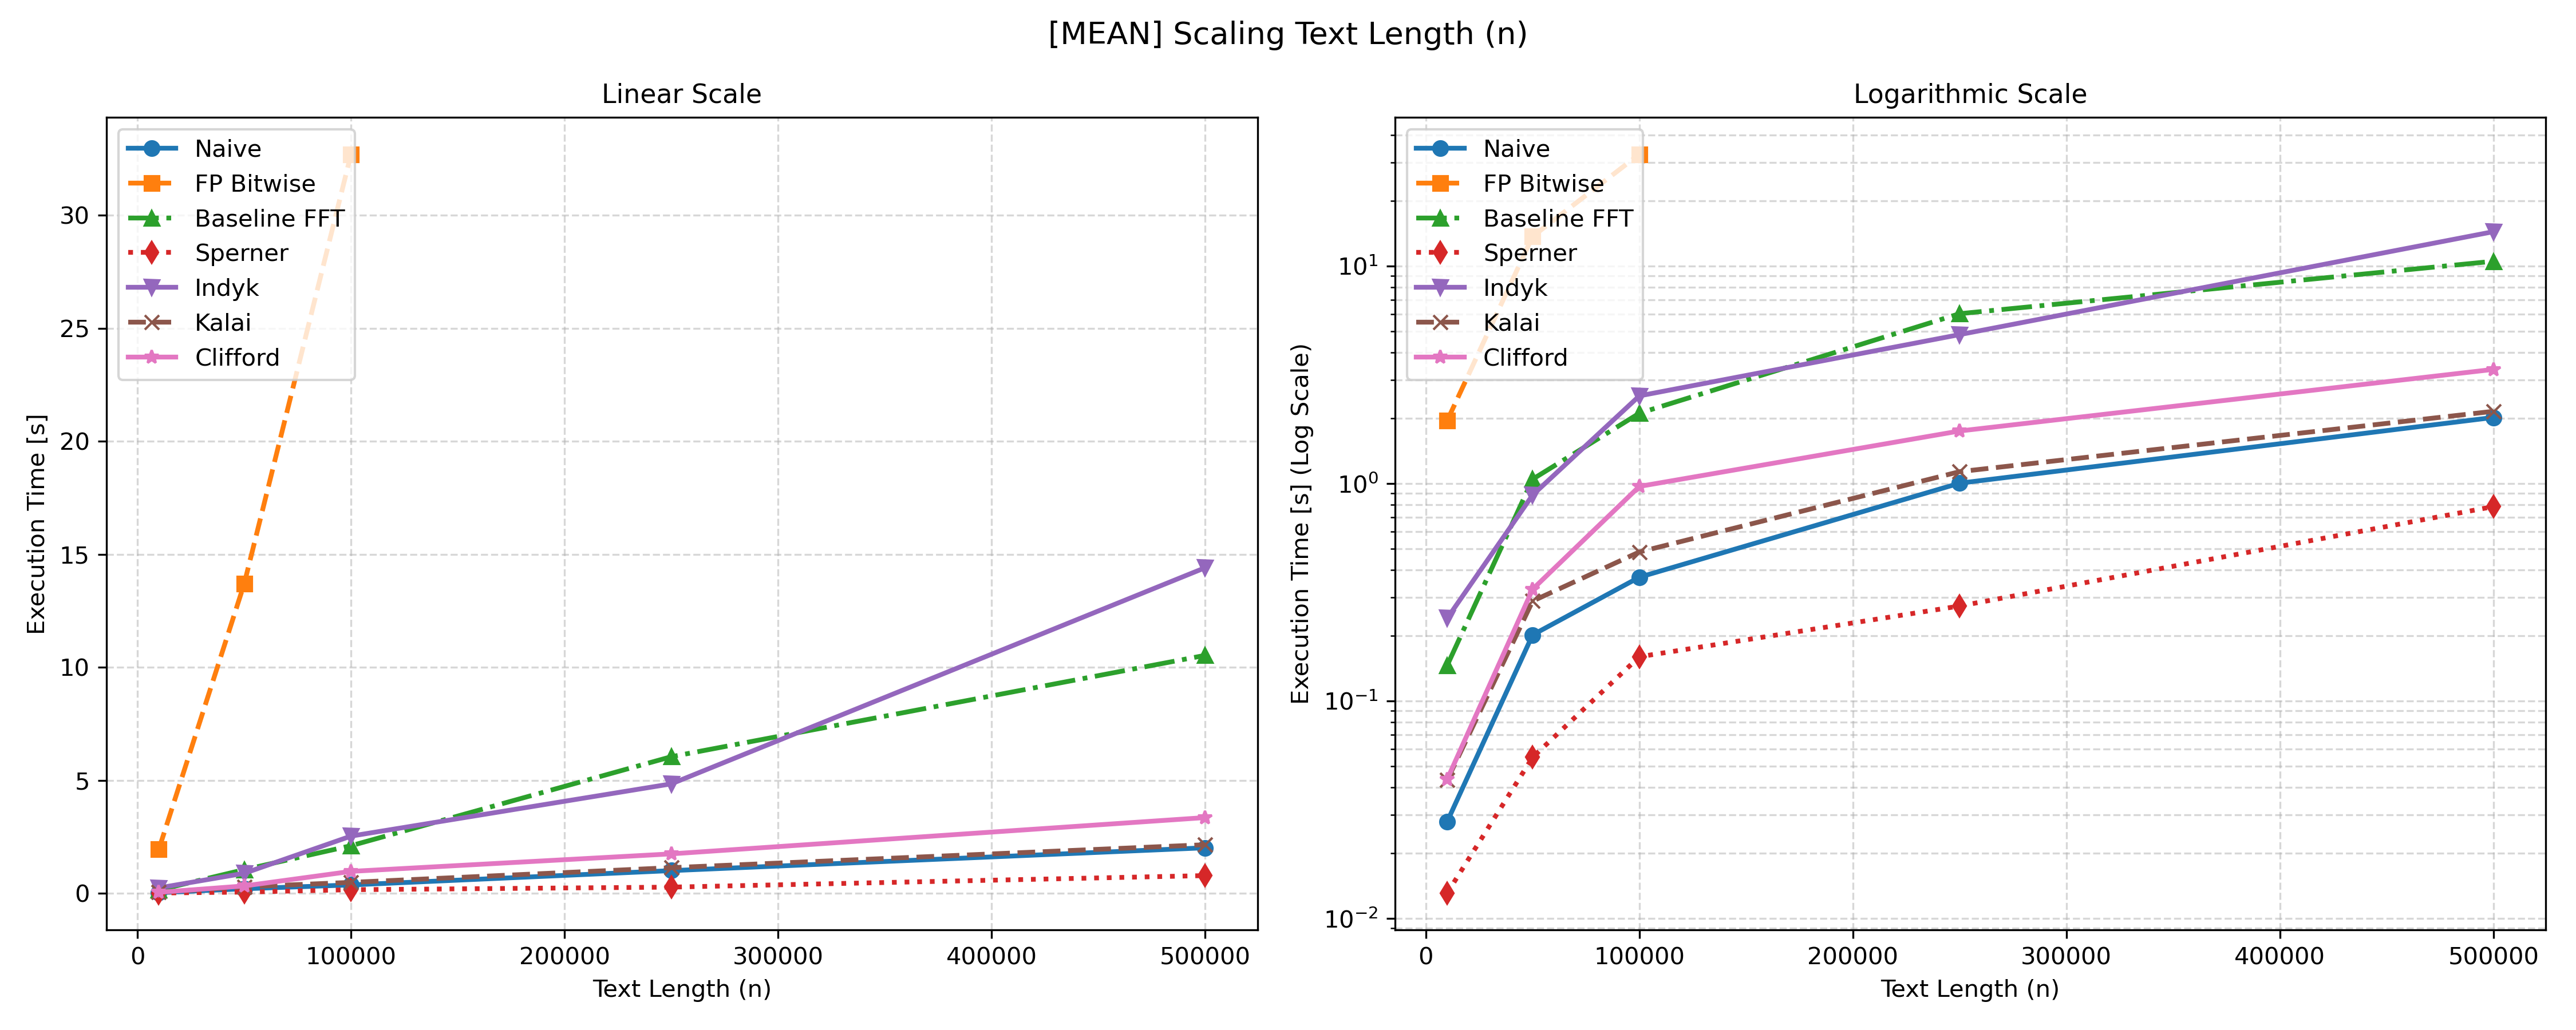
\includegraphics[width=\textwidth]{images/mean_plot_n.png}
    \caption{Scaling Text Length ($n$) under Average-Case conditions.}
    \label{fig:mean_n}
\end{figure}

Conversely, under worst-case inputs, every alignment forces the inner loop to scan through $m-1$ matching characters. As shown in Figure \ref{fig:worst_n}, the runtime increases drastically from $20.11$ seconds at $n=10000$ to over $366$ seconds at $n=100000$, after which it is safely omitted. This forms a sharp parabolic curve that confirms the exact $\mathcal{O}(nm)$ worst-case behavioral trap.

\begin{figure}[H]
    \centering
    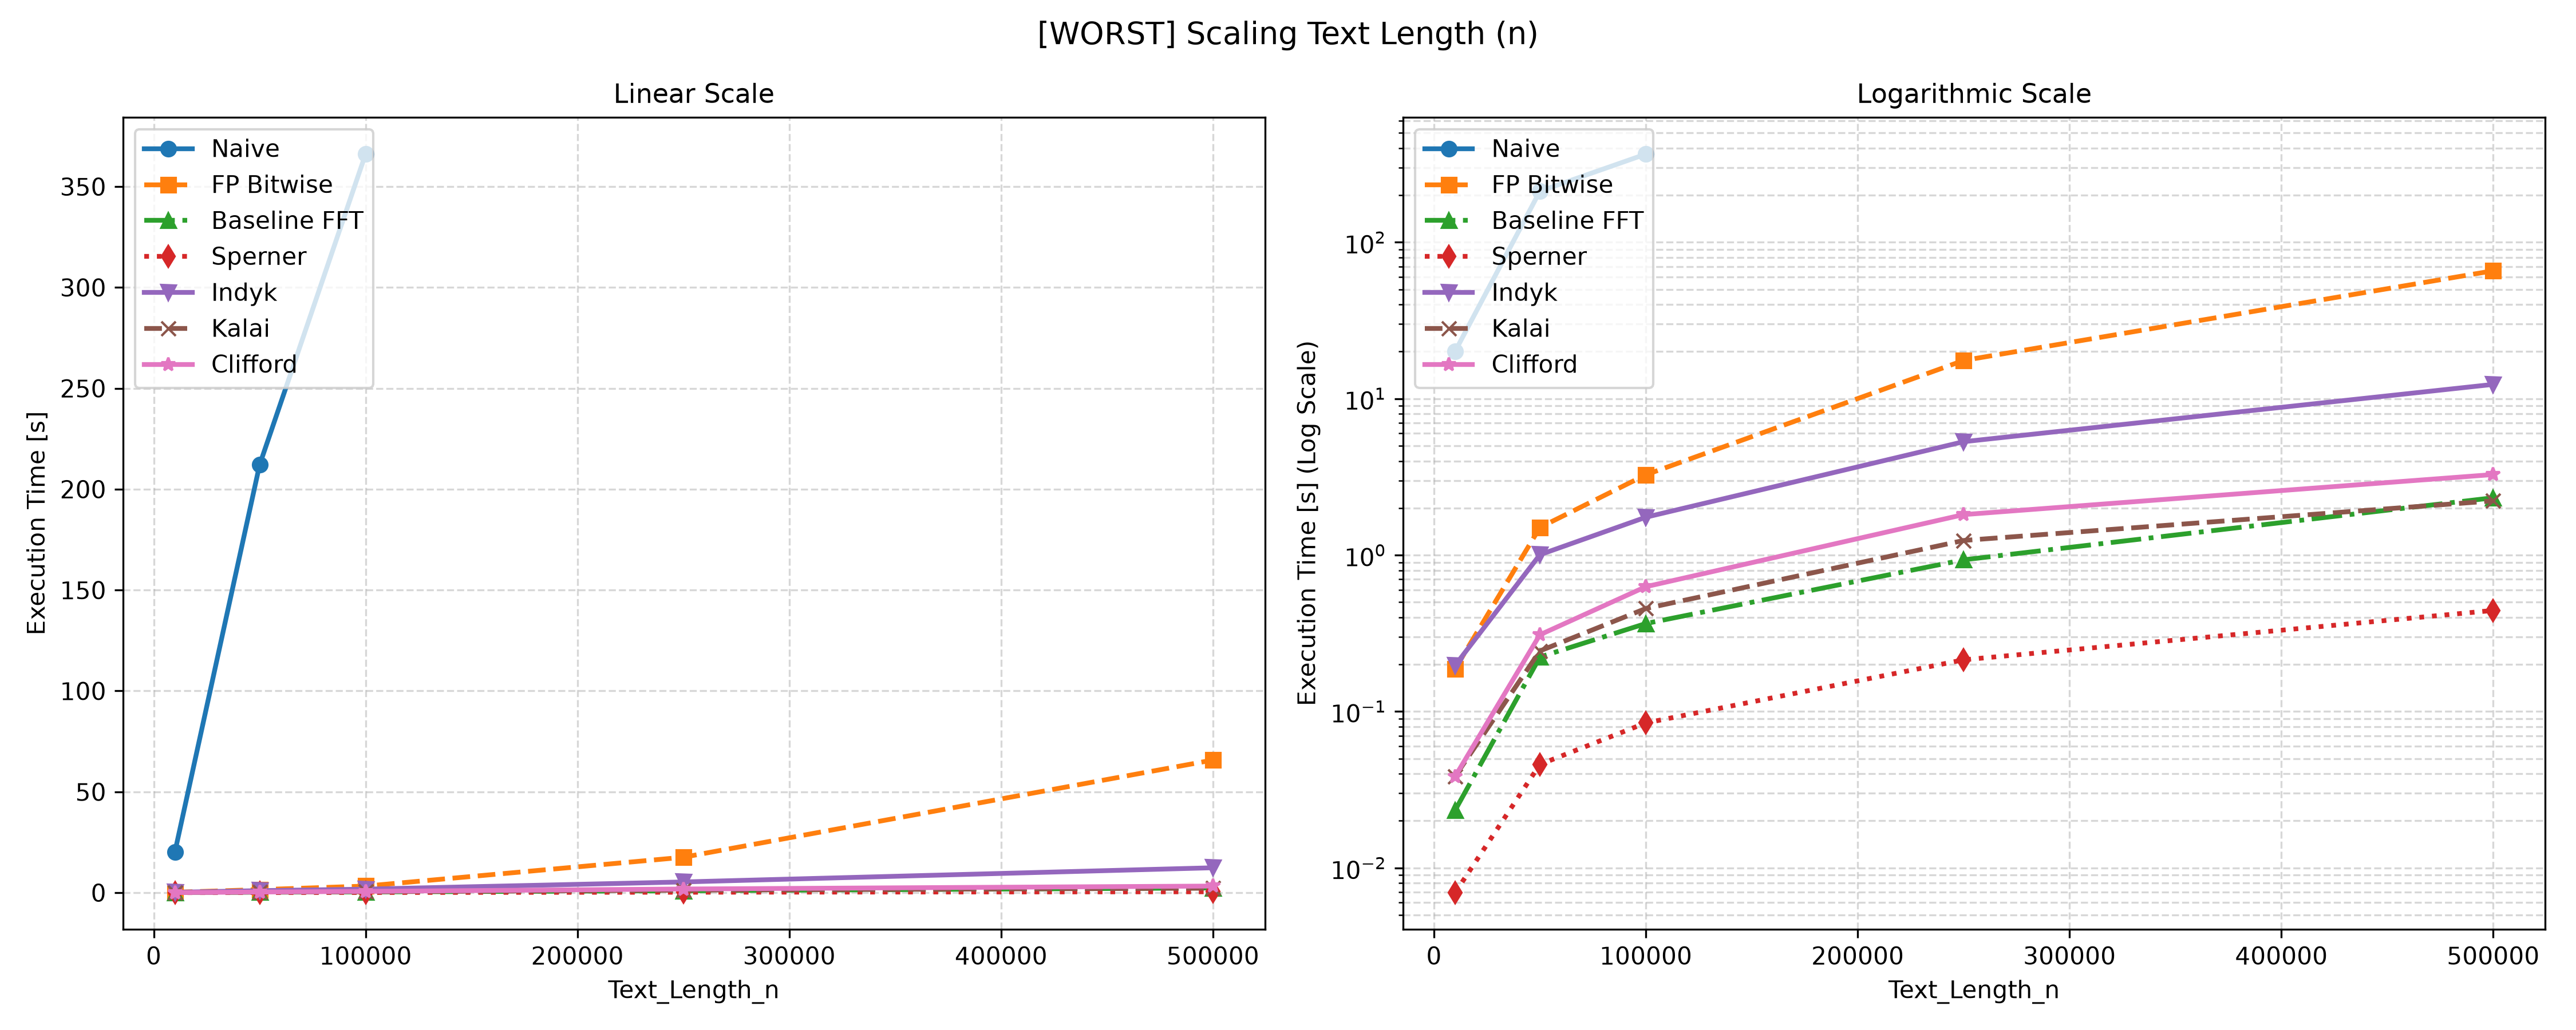
\includegraphics[width=\textwidth]{images/worst_plot_n.png}
    \caption{Scaling Text Length ($n$) under Worst-Case conditions.}
    \label{fig:worst_n}
\end{figure}

The structural degradation when scaling the pattern length $m$ (while holding the text length constant) fully mirrors the breakdown observed when scaling $n$. As shown in Figures \ref{fig:mean_m} and \ref{fig:worst_m}, increasing the pattern length matches the symmetric nature of the $\mathcal{O}(nm)$ worst-case boundary, while average-case execution remains mostly flat for the brute-force approach.

\begin{figure}[H]
    \centering
    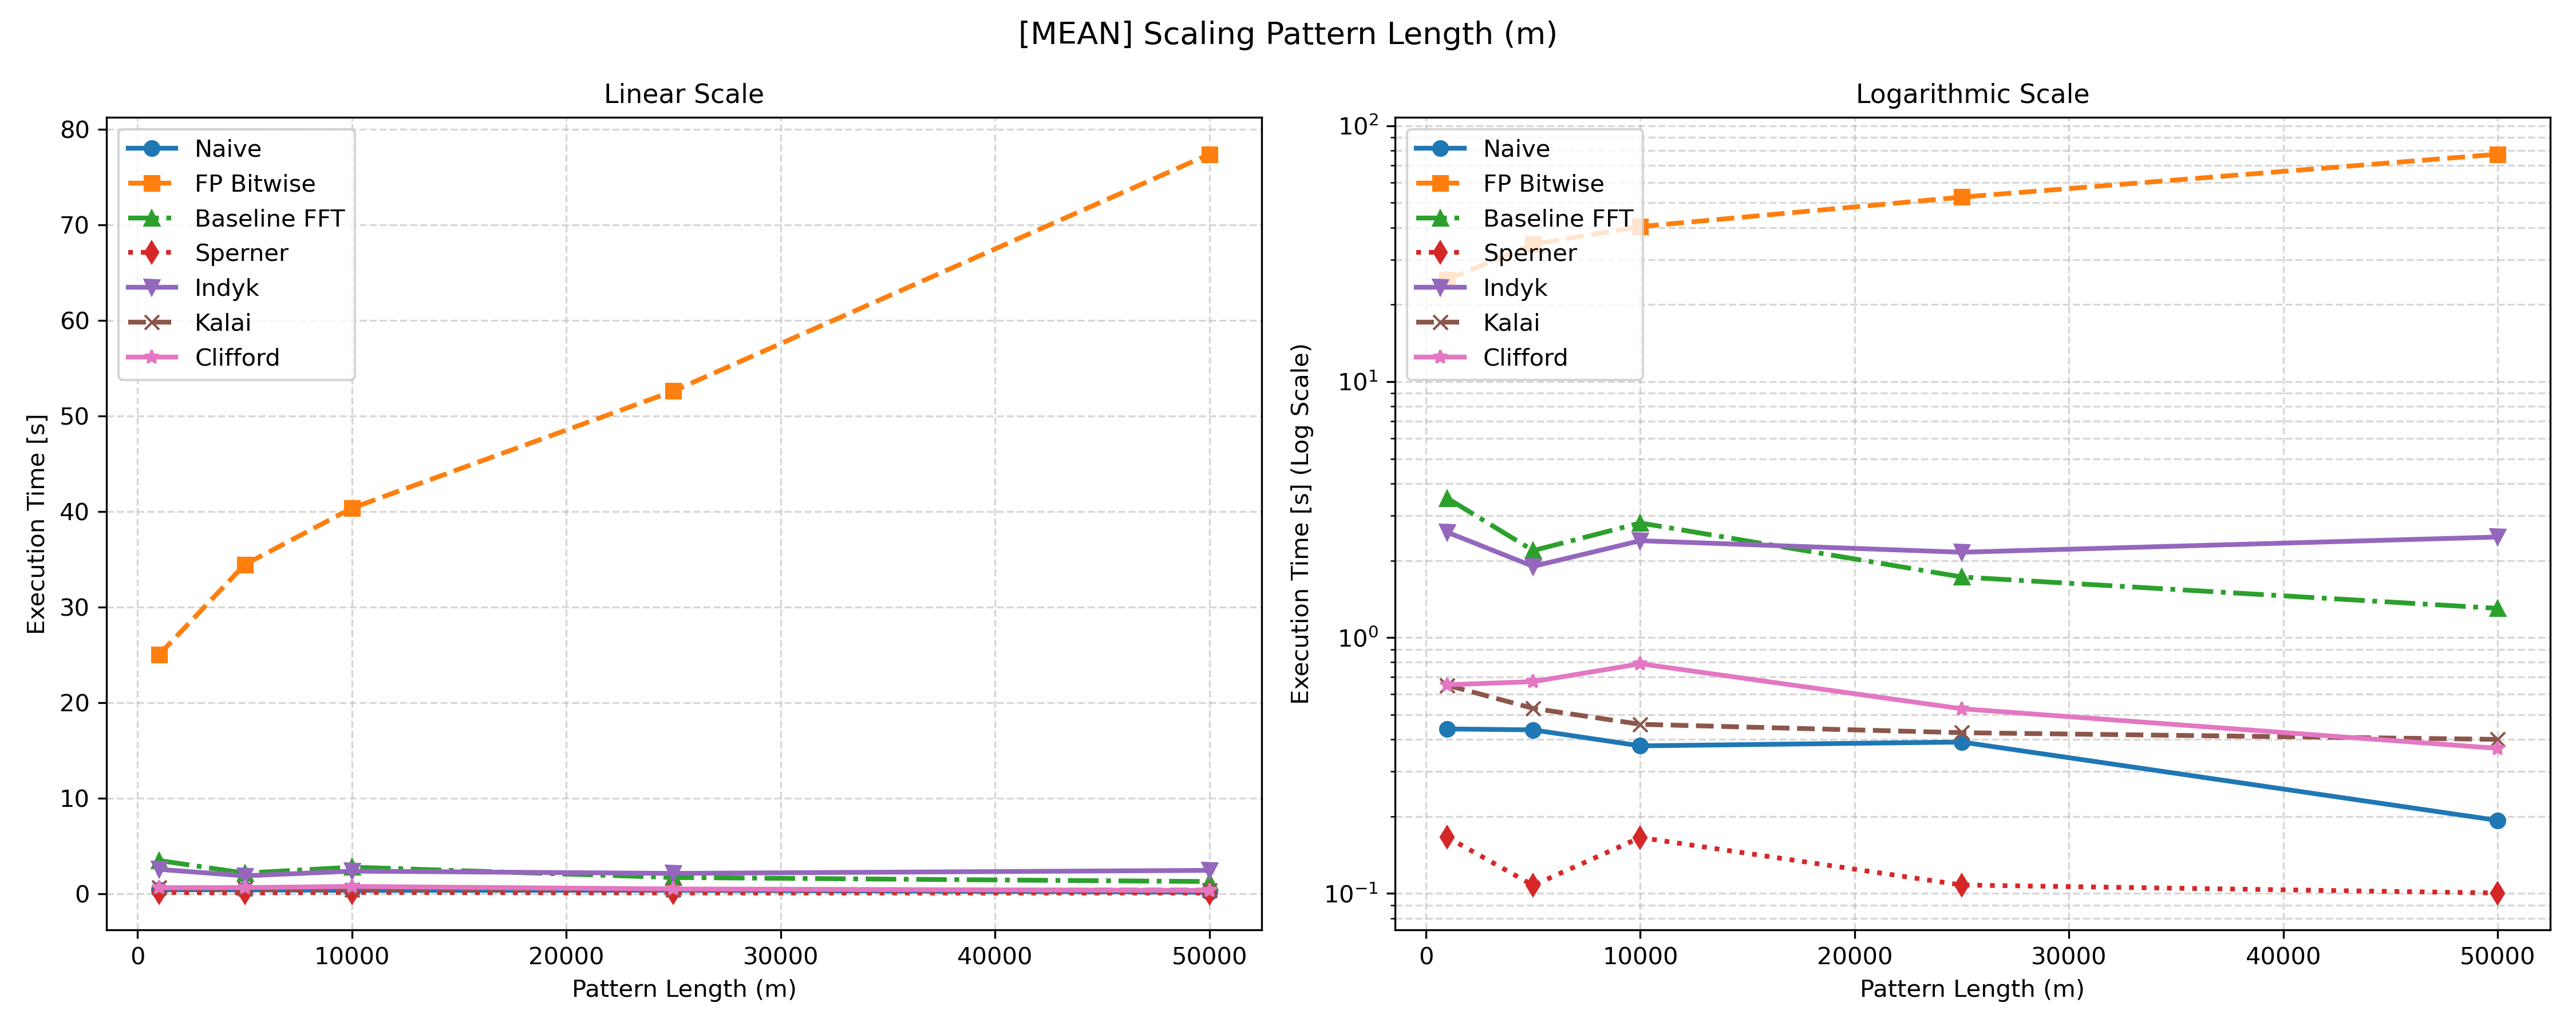
\includegraphics[width=\textwidth]{images/mean_plot_m.png}
    \caption{Scaling Pattern Length ($m$) under Average-Case conditions.}
    \label{fig:mean_m}
\end{figure}

\begin{figure}[H]
    \centering
    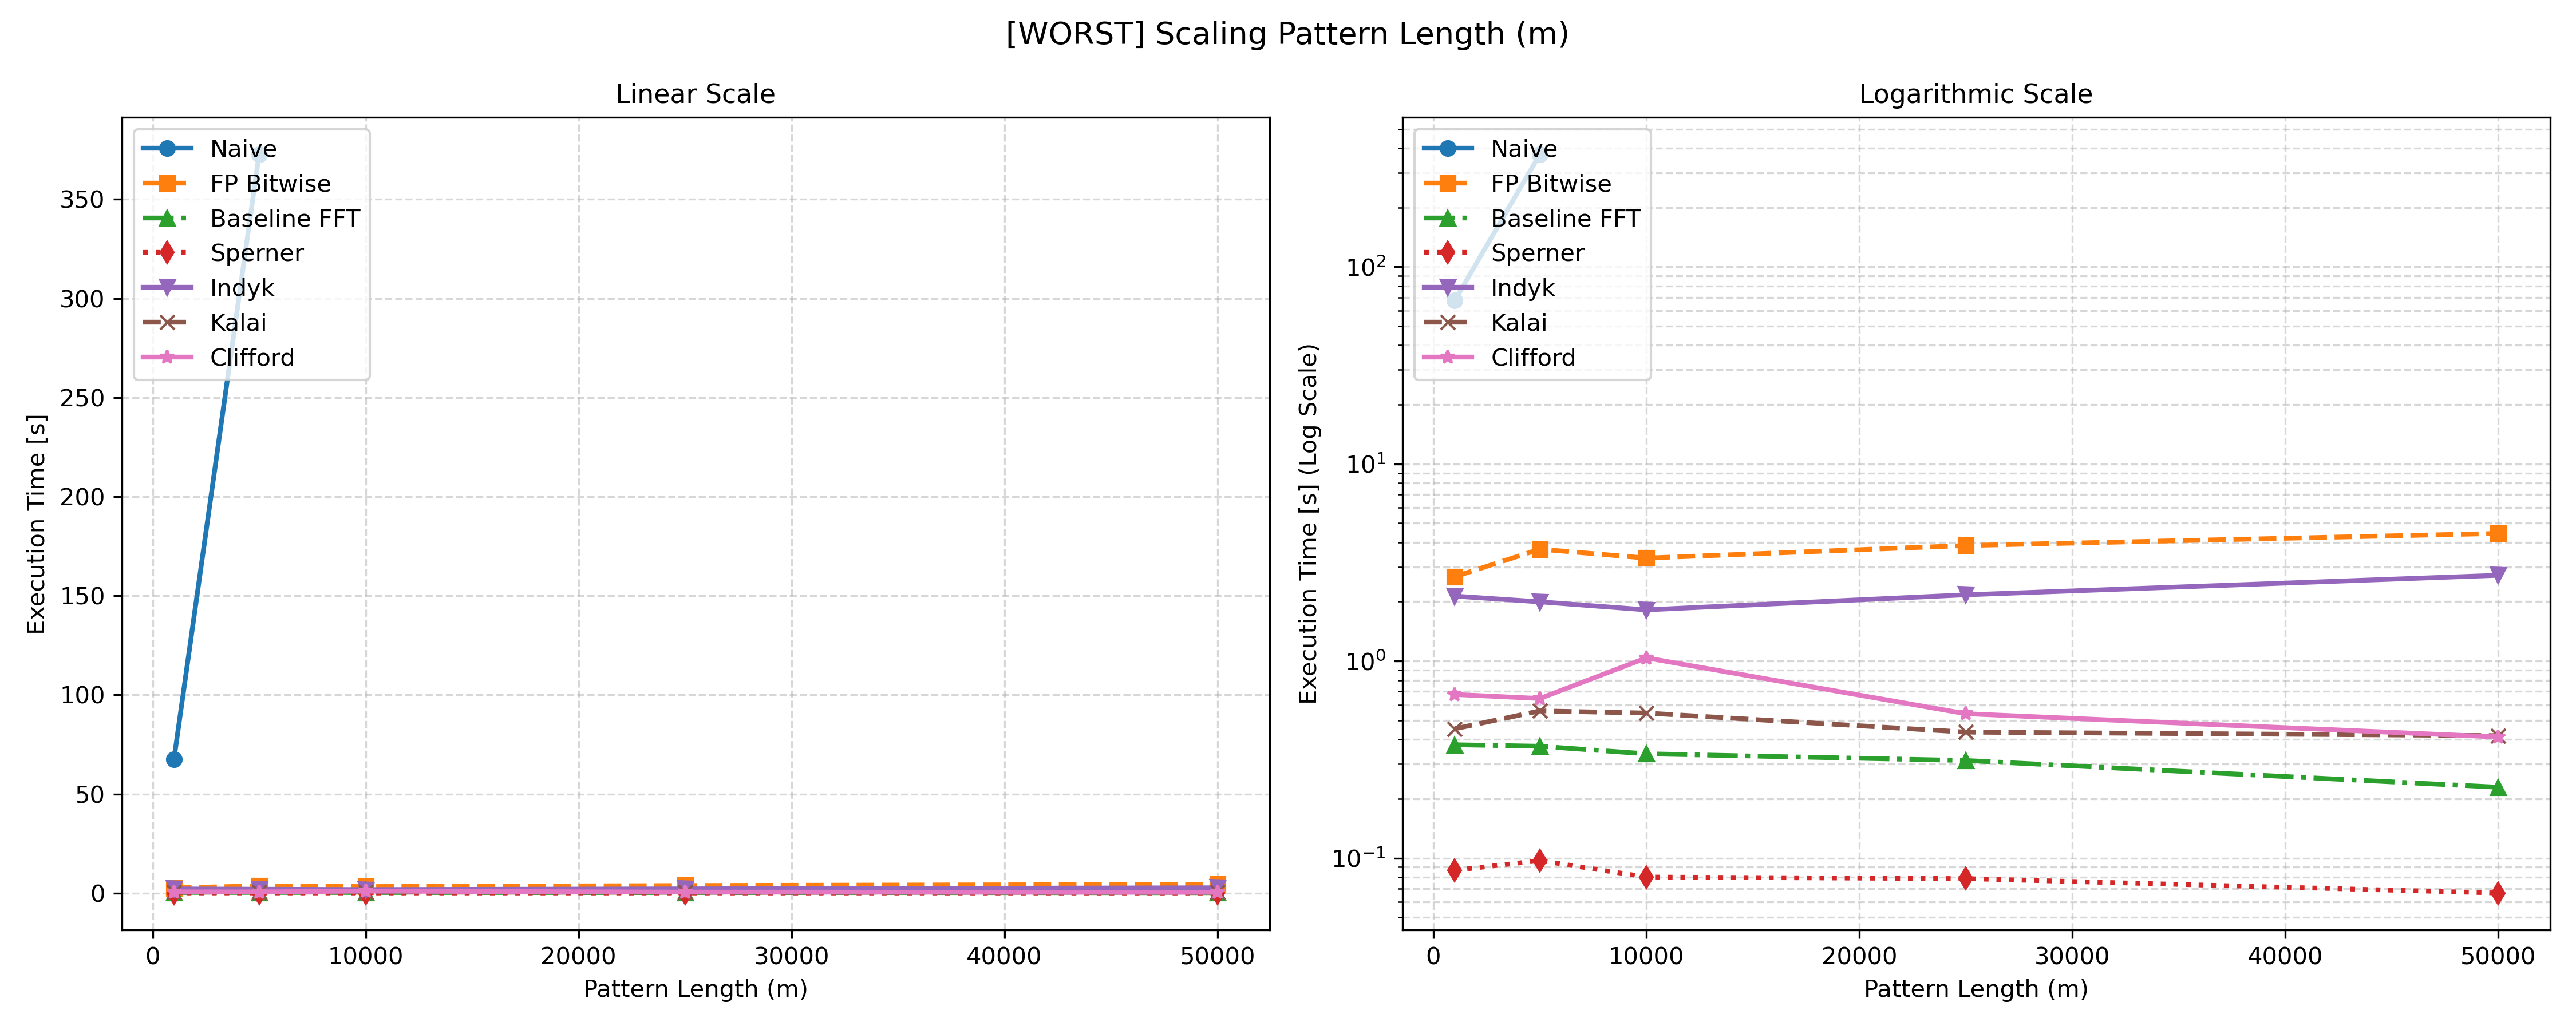
\includegraphics[width=\textwidth]{images/worst_plot_m.png}
    \caption{Scaling Pattern Length ($m$) under Worst-Case conditions.}
    \label{fig:worst_m}
\end{figure}

\section{Fischer-Paterson Bottleneck}
The Fischer-Paterson algorithm packs characters into large integers using bit shifts. The execution time depends heavily on the alphabet cardinality $|\Sigma|$ and the bit-length of the integer representations.

In the average-case test scaling the alphabet size (Figure \ref{fig:mean_sigma}), the presence of unique symbols forces the algorithm to execute Karatsuba multiplications over extremely large integers. This generates a significant polynomial performance degradation, where execution time surges to over $150$ seconds for an alphabet of $64$ symbols. 

\begin{figure}[H]
    \centering
    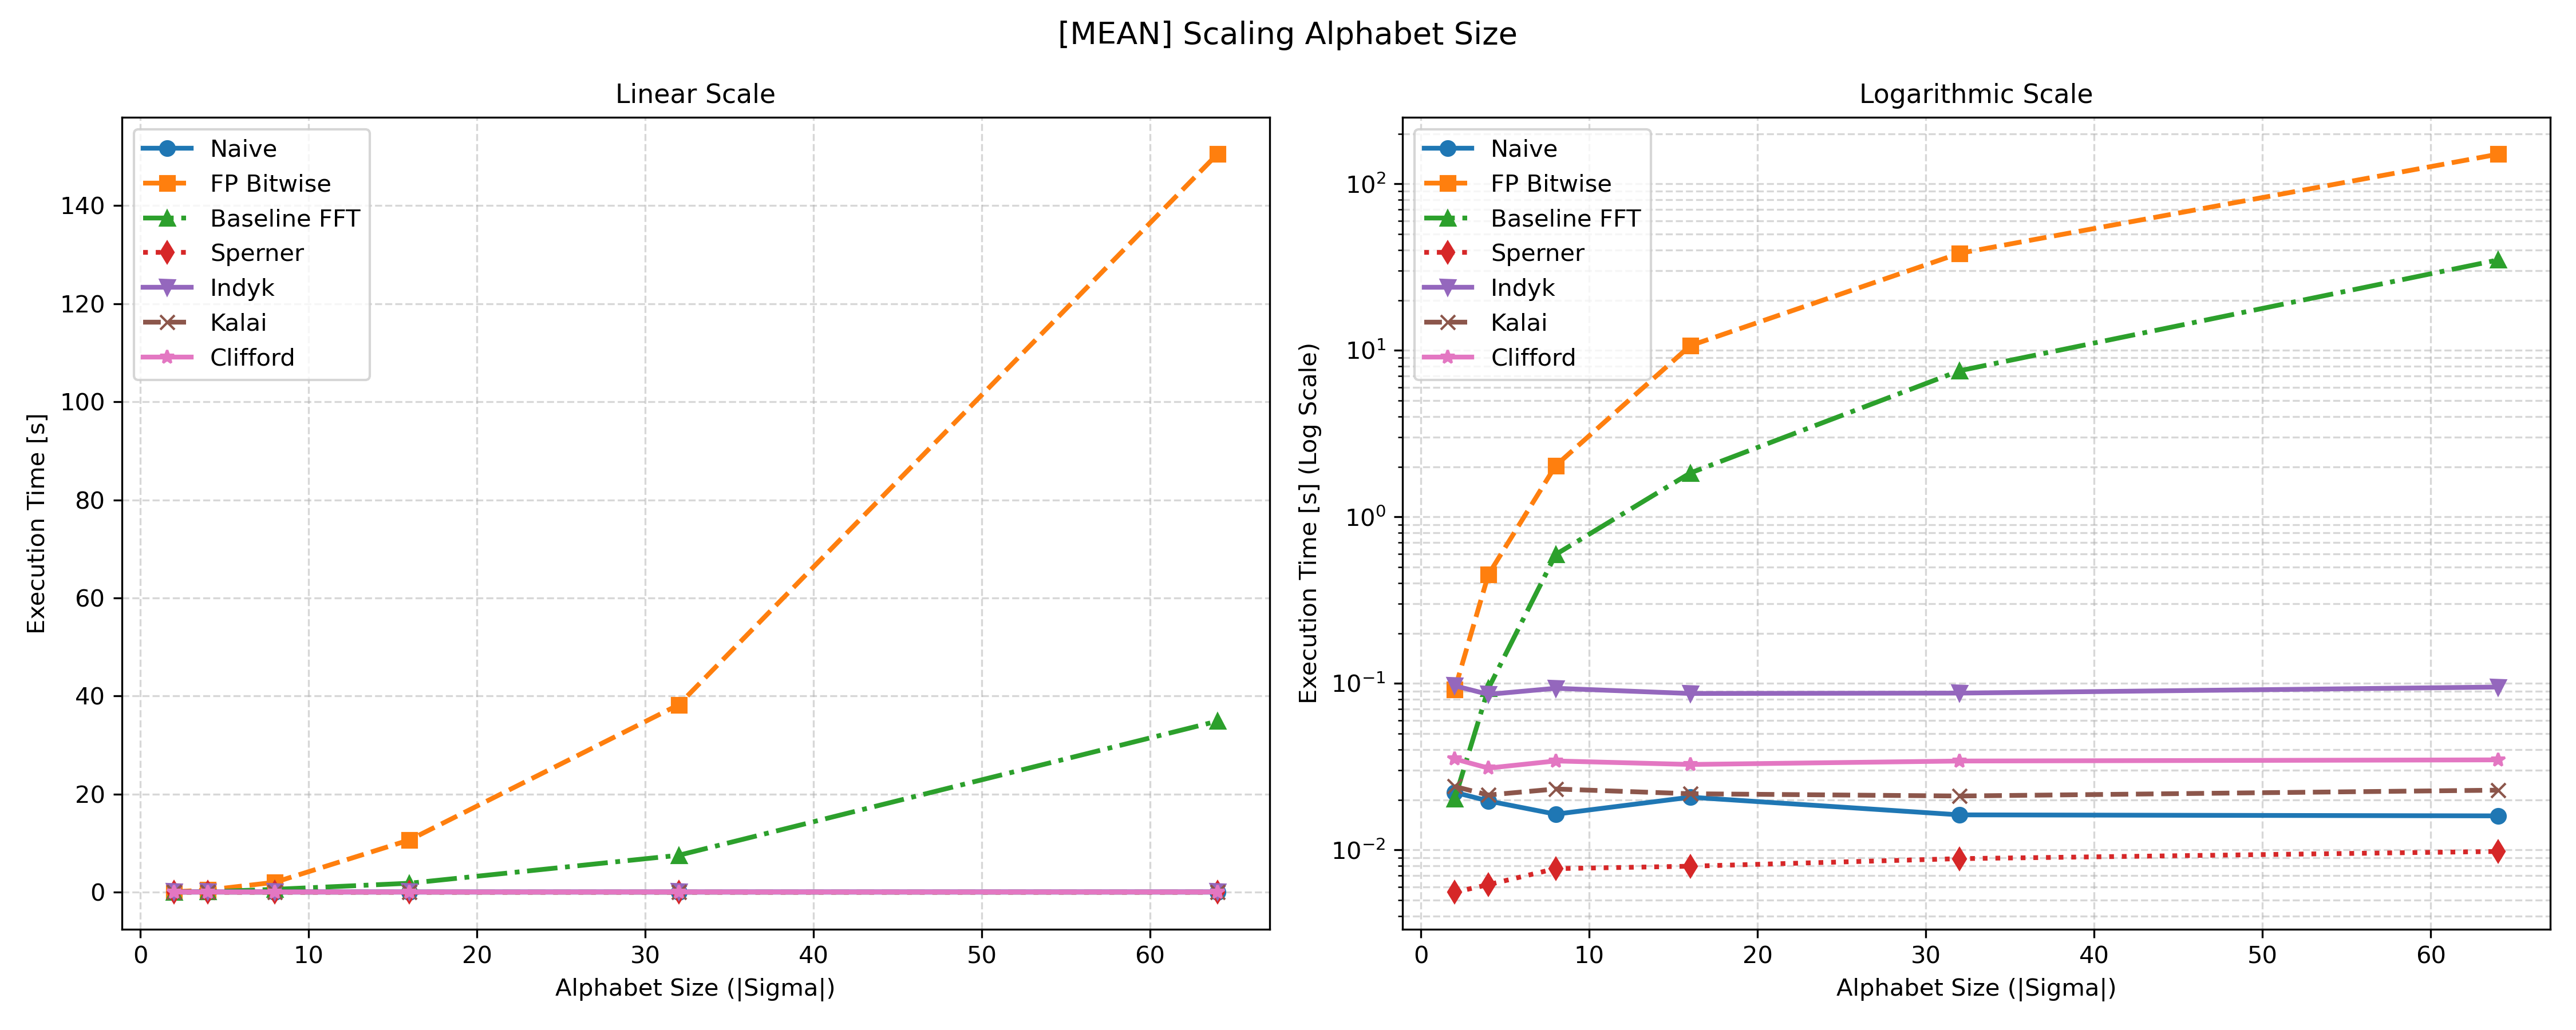
\includegraphics[width=\textwidth]{images/mean_plot_sigma.png}
    \caption{Scaling Alphabet Size ($|\Sigma|$) under Average-Case conditions.}
    \label{fig:mean_sigma}
\end{figure}

This exponential rise is uniquely bound to the FP Bitwise approach. As shown in the worst-case scaling (Figure \ref{fig:worst_sigma}), where the text is predominantly composed of a single repeating character, the arbitrary-precision multiplication completes significantly faster due to the lower variance in bits. More importantly, both figures firmly confirm that all modern FFT-based convolutions remain entirely decoupled from alphabet size constraints.

\begin{figure}[H]
    \centering
    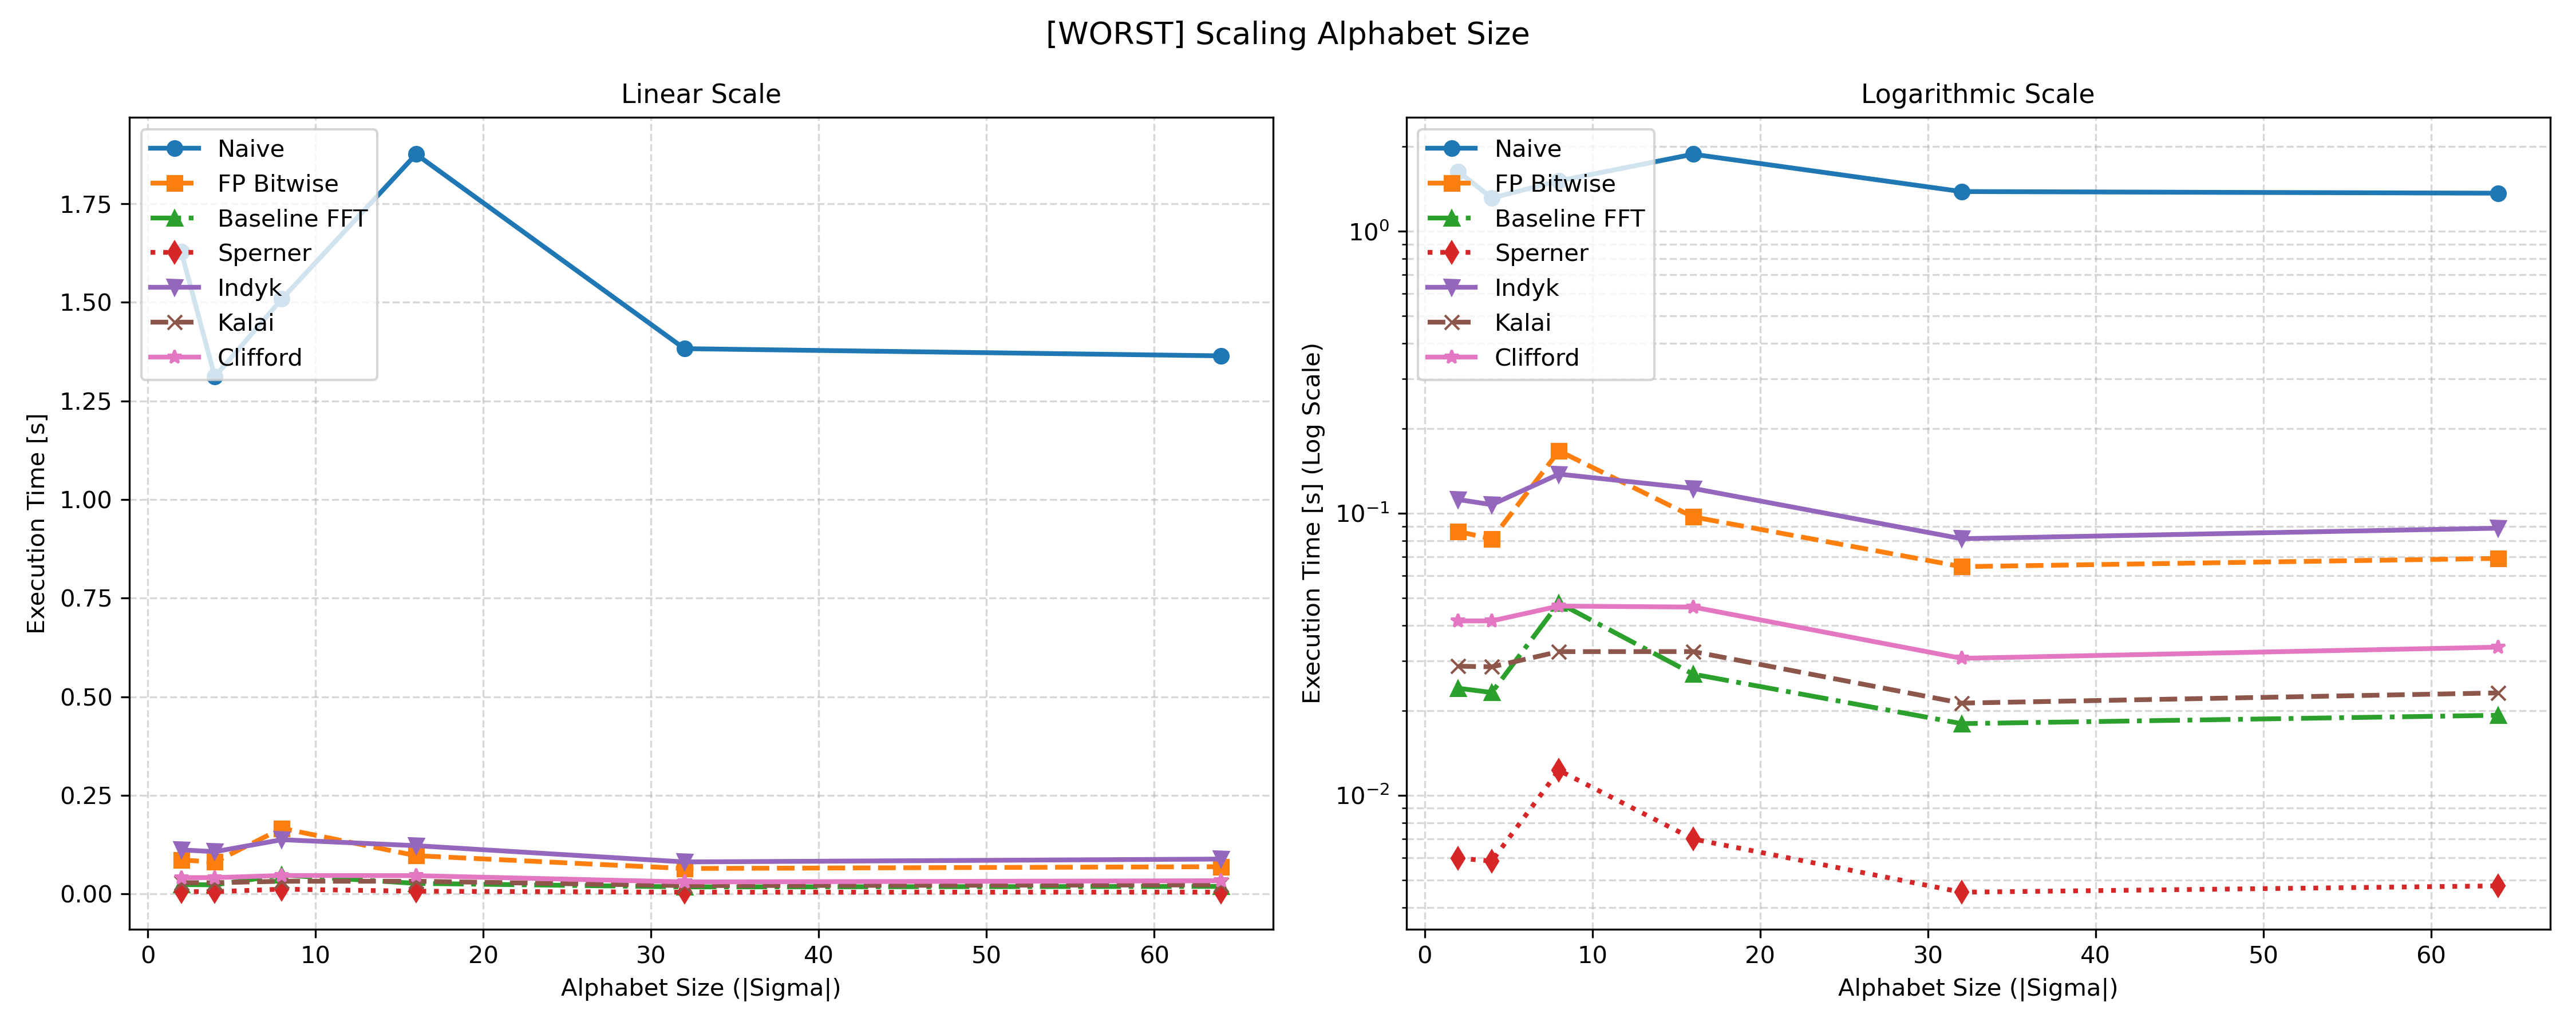
\includegraphics[width=\textwidth]{images/worst_plot_sigma.png}
    \caption{Scaling Alphabet Size ($|\Sigma|$) under Worst-Case conditions.}
    \label{fig:worst_sigma}
\end{figure}

\section{Constant Factors: Kalai, Indyk, and Clifford-Clifford}
Indyk, Kalai, and Clifford-Clifford all exhibit theoretically optimal or near-optimal asymptotic complexities. However, the benchmark plots reveal practical differences driven by their internal theoretical constant factors. 

For a large-scale text of length $n=500000$, Indyk takes $14.40$ seconds, Clifford-Clifford completes in $3.35$ seconds, and Kalai finishes natively in only $2.15$ seconds. 

This performance hierarchy aligns perfectly with their underlying algebraic structures:
\begin{itemize}
    \item \textbf{Kalai (Probabilistic Optimal):} Requires exactly two forward FFTs and two inverse FFTs per search ($C_{\text{Kalai}} = 4 \cdot \mathcal{F}(L)$). This light constant factor makes it the fastest among the advanced convolution algorithms, though it inherently carries a mathematically bounded $\mathcal{O}(1/n)$ error risk.
    \item \textbf{Clifford-Clifford (Deterministic Optimal):} Evaluates the exact Euclidean distance using exactly three FFT passes on squared and cubed numerical arrays. Generating these high-power algebraic vectors and managing block-overlaps introduces a slightly heavier constant factor than Kalai, but it successfully eliminates the probabilistic error risk, making it the most efficient purely deterministic solution.
    \item \textbf{Indyk (Randomized Projections):} To keep the false-positive rate sufficiently low, it performs $d = c \cdot \log_2(n)$ independent projection dimensions. For large text inputs, this requires generating multiple independent trials and executing dozens of physical FFT operations sequentially. This severely penalizes the algorithm's practical runtime despite its theoretical $\mathcal{O}(n \log n)$ boundary.
\end{itemize}

\section{Proportional Asymptotic Scaling}
To directly observe theoretical boundaries, the proportional scaling test continuously increases the pattern length as $m = 0.1n$. This forces the algorithmic product $n \cdot m$ to grow quadratically, while $\mathcal{O}(n \log n)$ grows marginally faster than linearly. 

As captured in Figure \ref{fig:prop_nm}, the \textsc{Naive} algorithm forms a steep parabolic trajectory, reaching over $170$ seconds at $n=50000$. Meanwhile, the FFT-based algorithms appear completely flat on the linear scale. The logarithmic right panel reveals their true logarithmic progression, fitting the algebraic scalability proofs established by Kalai, Indyk, and Clifford-Clifford. Both Kalai and Clifford-Clifford finish in roughly $3$ seconds at $n=400000$, maintaining nearly parallel trajectories that match their tight $\mathcal{O}(n \log m)$ bounds.

\begin{figure}[H]
    \centering
    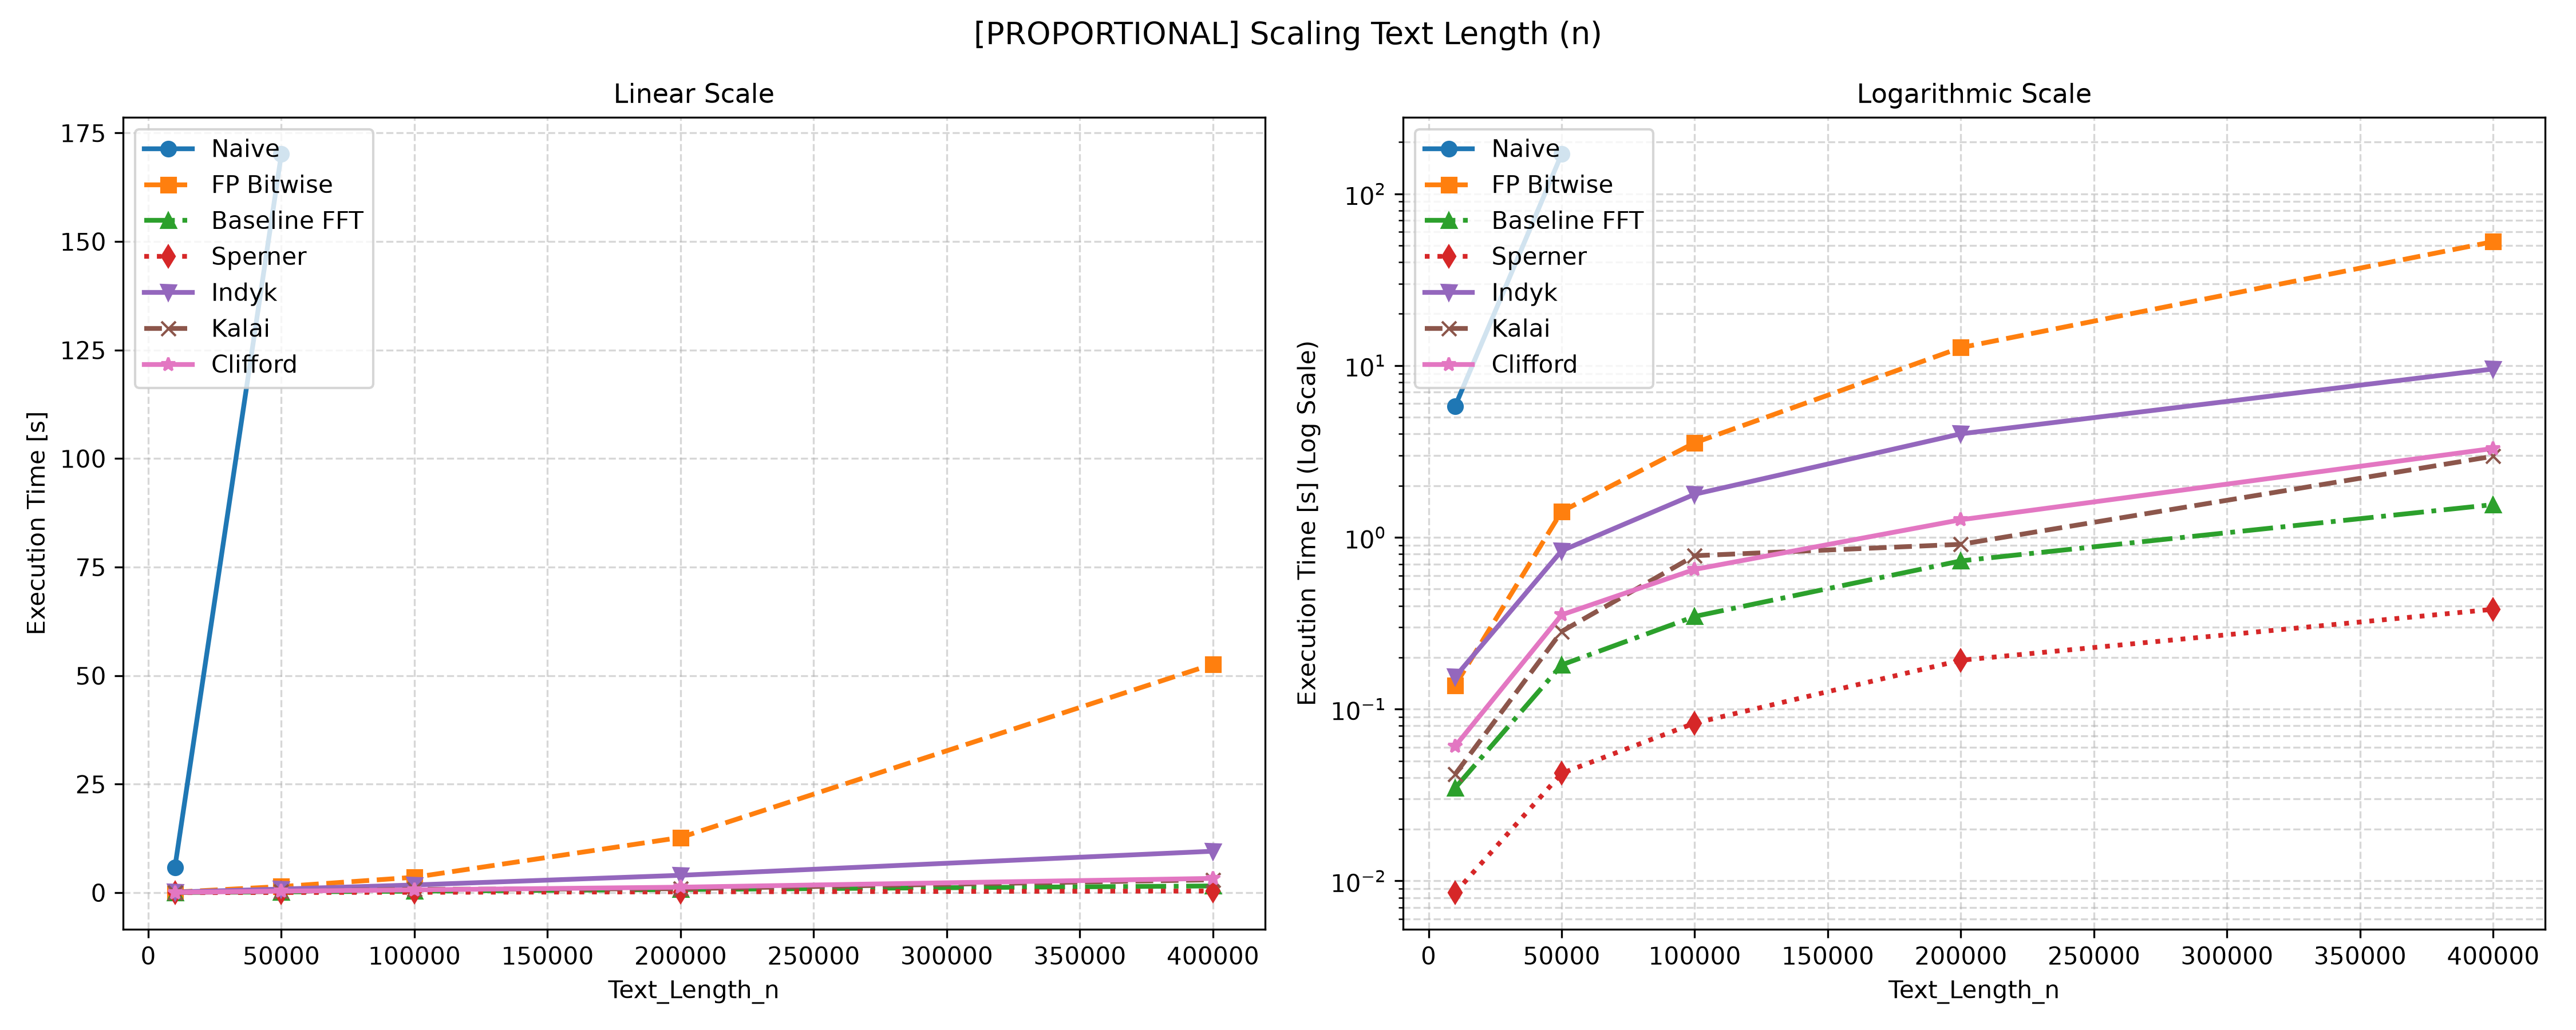
\includegraphics[width=\textwidth]{images/proportional_plot_nm.png}
    \caption{Proportional Scale Test proving $\mathcal{O}(n^2)$ vs $\mathcal{O}(n \log n)$ bounds.}
    \label{fig:prop_nm}
\end{figure}
\section{Wildcard Saturation}
The wildcard saturation experiment (Figure \ref{fig:density}) evaluates algorithm behavior as the wildcard density $p$ scales from $0\%$ to $50\%$. 

For the \textsc{Naive} algorithm, the execution time nearly doubles as the wildcard density grows (scaling from roughly $0.35$ to $0.60$ seconds). While this difference appears minimal on the macro scale, it exposes a fundamental structural vulnerability. Because the wildcard symbol mathematically guarantees a local match, a higher density prevents the algorithm's inner loop from breaking early upon encountering a mismatch. Consequently, the algorithm is forced to scan deeper into the pattern at every shift, directly increasing the total number of character comparisons.

\begin{figure}[H]
    \centering
    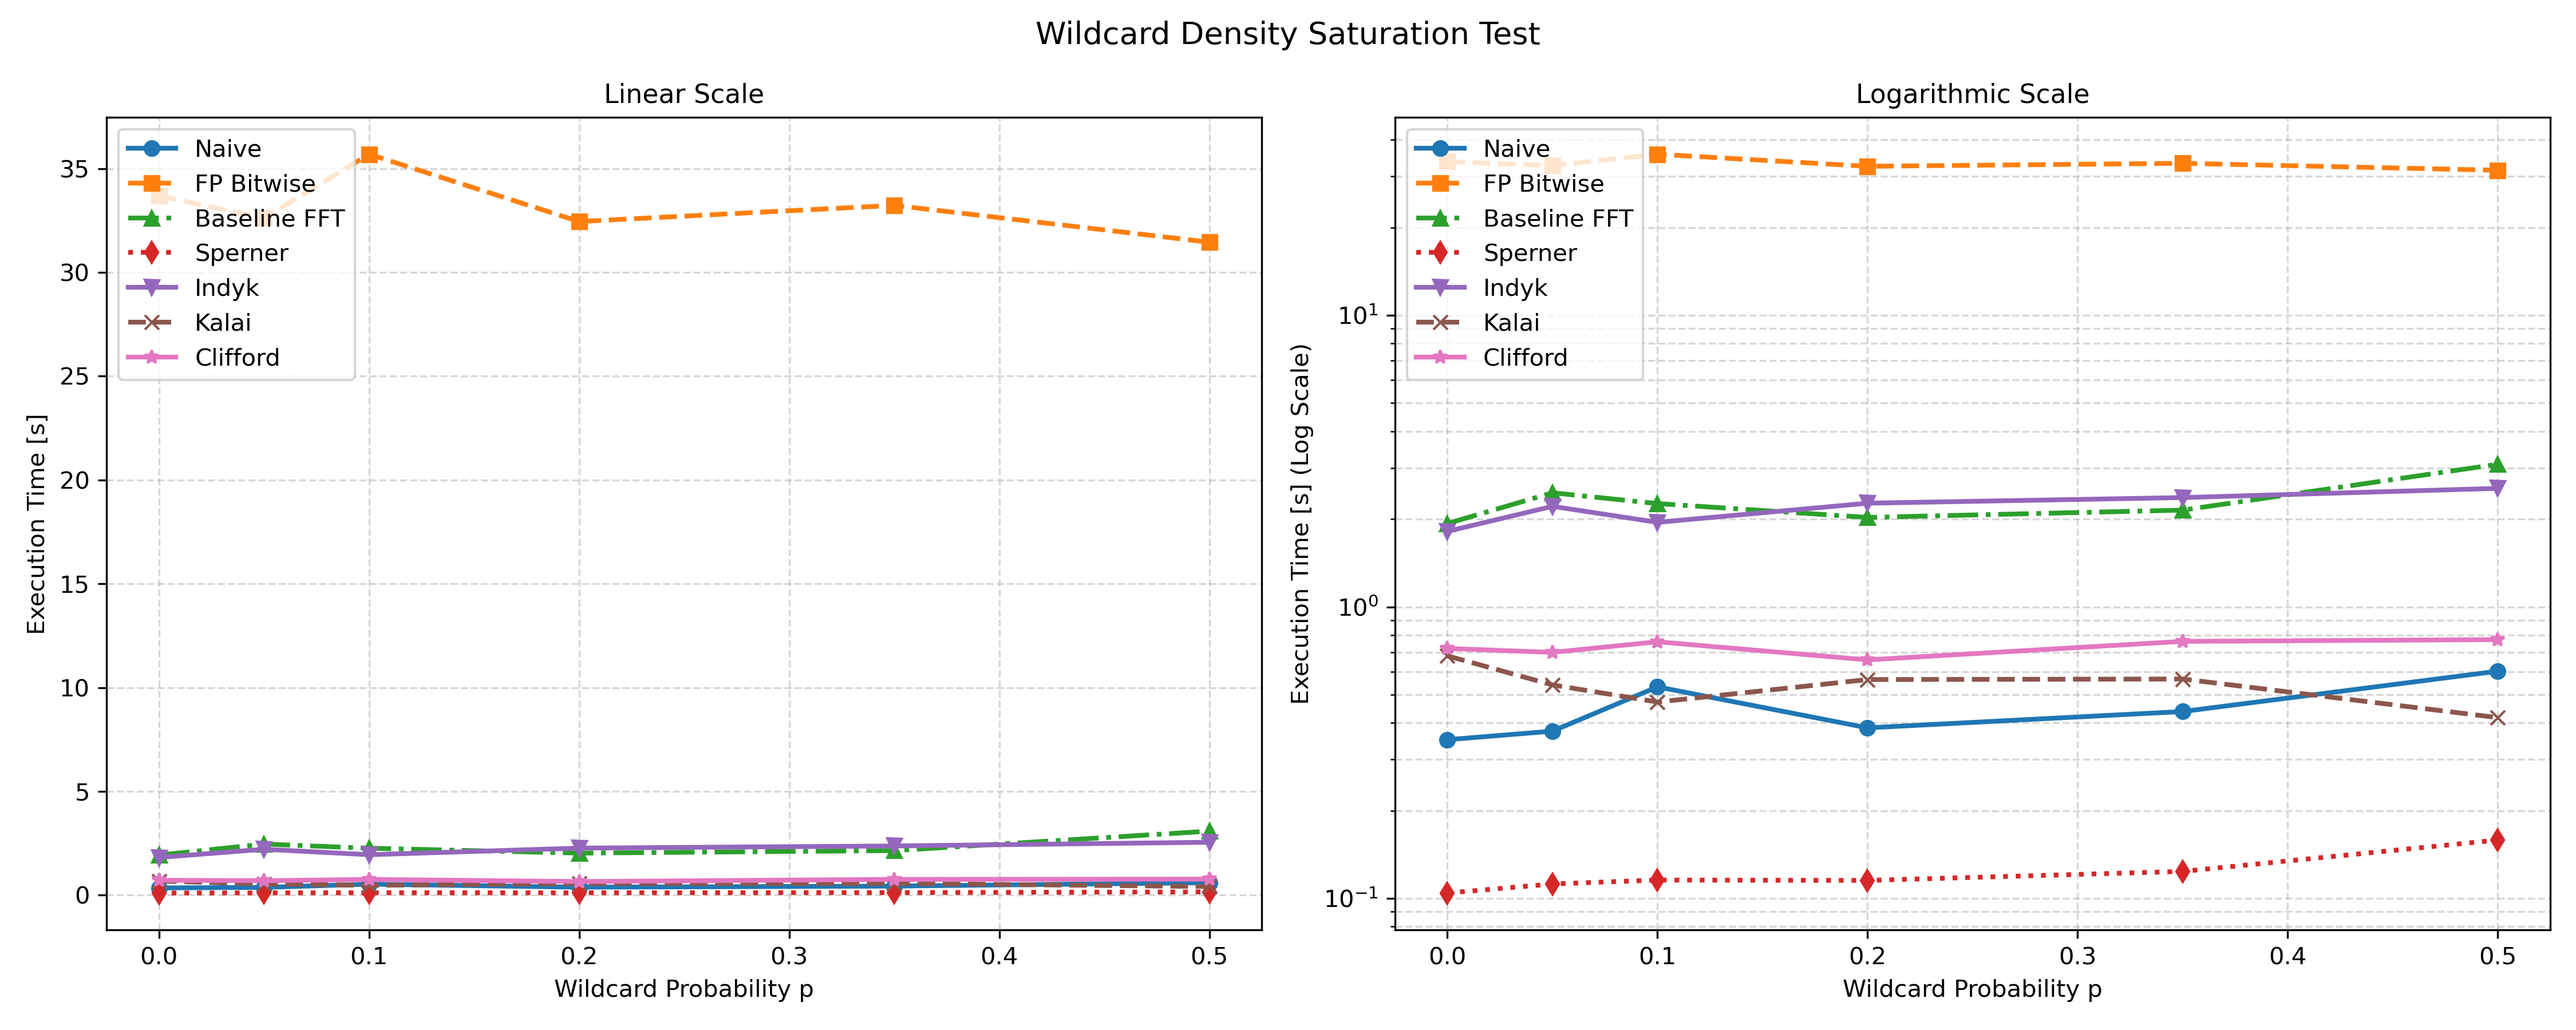
\includegraphics[width=\textwidth]{images/plot_wildcard_density.png}
    \caption{Wildcard Density Saturation Test.}
    \label{fig:density}
\end{figure}

In contrast, all convolution-based approaches remain stable because the required vector operations and FFT transforms are identical regardless of the input characters. With the array dimensions and the number of complex multiplications remaining constant, the presence of wildcards does not affect their execution speed.
\chapter{Conclusion and Summary}

This research confirms that while Fischer and Paterson established the theoretical foundations for string matching with wildcards, practical modern implementations heavily rely on Fast Fourier Transforms. Empirical verification with randomized trials throughout this research detected zero false positives, supporting the claim that the mathematical bounds established for Indyk's and Kalai's probabilistic methods hold consistently in practice.

To synthesize the theoretical complexities, empirical timings, and memory trade-offs evaluated in this research, a practical comparative overview for future software implementations is provided below:

\begin{itemize}
    \item \textbf{Naive:} This method is ideal for short patterns ($m < 32$) and small natural text alphabets. It requires zero heap allocation and offers excellent cache locality. However, its efficiency degrades significantly to $\mathcal{O}(nm)$ when processing dense wildcards or repetitive data sets.
    
    \item \textbf{FP Bitwise:} Serving primarily as a historical academic baseline, this method relies strictly on pure integer arithmetic. It is severely limited by the $\mathcal{O}(|\Sigma|^2)$ overhead generated by arbitrary-precision multiplication.
    
    \item \textbf{Baseline FFT:} Highly effective for data streams built on small alphabets (such as DNA, where $|\Sigma| \le 4$), delivering exact and fully deterministic matches. Its execution overhead is linearly dependent on the size of the underlying alphabet.
    
    \item \textbf{Sperner:} Designed for strictly deterministic applications requiring absolute certainty. It guarantees algorithmic performance mathematically bounded by a logarithmic alphabet scaling of $\mathcal{O}(\log |\Sigma|)$. Implementing it introduces mild combinatorial overhead needed for dynamic subset generation.
    
    \item \textbf{Indyk:} Suitable for traversing large character sets such as Unicode. It is asymptotically almost optimal, operating in $\mathcal{O}(n \log n)$ time, completely independent of the alphabet size. In practical software, however, it is burdened by a high constant factor generated by the need to compute independent FFT passes per validation.
    
    \item \textbf{Kalai:} A highly efficient architectural choice for practical applications requiring fast convolutions. It maintains a minimum constant factor of exactly 4 FFT iterations, ensuring execution speeds bounded by $\mathcal{O}(n \log m)$. It requires system infrastructure explicitly tolerant of Monte Carlo false positive rates capped at $\le 1/N$.
    
    \item \textbf{Clifford-Clifford:} The optimal choice for purely deterministic $\mathcal{O}(n \log m)$ pattern matching. By expanding Euclidean distance into three separate transforms, it provides absolute accuracy independent of the alphabet size, avoiding probabilistic errors at the cost of a slightly heavier constant factor than Kalai.
\end{itemize}

The empirical results definitively show that the Fast Fourier Transform fundamentally restructures wildcard string matching, providing robust scalability for modern data environments.

\clearpage
\phantomsection
\addcontentsline{toc}{chapter}{References}
\bibliographystyle{plain}
\bibliography{references}

\vspace{1cm}
\noindent \textit{Note: In accordance with Jagiellonian University's Regulation No. 115/2025, Large Language Models (LLMs) were utilized during the preparation of this work strictly for English language proofreading, stylistic refinement, and LaTeX typesetting assistance.}

\clearpage
\appendix
\appendix
\chapter{Raw Benchmark Data}
\label{sec:appendix_data}

This appendix presents the numerical execution times collected during the empirical evaluation. Each measurement was repeated 5 times, and the values reported in the tables below represent the median runtime across those iterations. Entries marked as \texttt{TLE} (Time Limit Exceeded) indicate that the execution was terminated after exceeding the predefined benchmark time limit.

\section{Text Length ($n$) and Proportional Scaling}

\begin{table}[H]
\centering
\caption{Execution time (s) scaling text length $n$ (Average-Case, $m=5000, |\Sigma|=4$).}
\label{tab:mean_n_data}
\begin{tabular}{@{}lrrrrrrrr@{}}
\toprule
$n$ & Naive & FP Bitwise & Baseline FFT & Sperner & Indyk & Kalai & Clifford \\
\midrule
10000  & 0.028 & 1.948 & 0.146 & 0.013 & 0.240 & 0.043 & 0.044 \\
50000  & 0.201 & 13.696 & 1.047 & 0.055 & 0.886 & 0.288 & 0.327 \\
100000 & 0.371 & 32.694 & 2.106 & 0.160 & 2.531 & 0.485 & 0.970 \\
250000 & 1.004 & {\footnotesize TLE}   & 6.043 & 0.273 & 4.842 & 1.134 & 1.745 \\
500000 & 2.014 & {\footnotesize TLE}   & 10.526 & 0.783 & 14.401 & 2.149 & 3.350 \\
\bottomrule
\end{tabular}
\end{table}

\begin{table}[H]
\centering
\caption{Execution time (s) scaling text length $n$ (Worst-Case, $m=5000, |\Sigma|=4$).}
\label{tab:worst_n_data}
\begin{tabular}{@{}lrrrrrrrr@{}}
\toprule
$n$ & Naive & FP Bitwise & Baseline FFT & Sperner & Indyk & Kalai & Clifford \\
\midrule
10000  & 20.112 & 0.187 & 0.023 & 0.007 & 0.197 & 0.039 & 0.038 \\
50000  & 212.103 & 1.502 & 0.223 & 0.046 & 1.006 & 0.244 & 0.309 \\
100000 & 366.096 & 3.261 & 0.365 & 0.085 & 1.746 & 0.456 & 0.628 \\
250000 & {\footnotesize TLE}    & 17.554   & 0.933 & 0.214 & 5.310 & 1.240 & 1.815 \\
500000 & {\footnotesize TLE}    & 65.743   & 2.326 & 0.443 & 12.342 & 2.222 & 3.274 \\
\bottomrule
\end{tabular}
\end{table}

\begin{table}[H]
\centering
\caption{Proportional Scaling $m = 0.1n$ (Worst-Case, $|\Sigma|=4$).}
\label{tab:prop_nm_data}
\begin{tabular}{@{}lrrrrrrrr@{}}
\toprule
$n$ & $m$ & Naive & FP Bitwise & Baseline FFT & Sperner & Indyk & Kalai & Clifford \\
\midrule
10000  & 1000 & 5.810  & 0.138 & 0.035 & 0.009 & 0.154 & 0.042 & 0.061 \\
50000  & 5000 & 170.136 & 1.414 & 0.181 & 0.042 & 0.835 & 0.283 & 0.354 \\
100000 & 10000 & {\footnotesize TLE}   & 3.552 & 0.347 & 0.083 & 1.783 & 0.782 & 0.651 \\
200000 & 20000 & {\footnotesize TLE}   & 12.720   & 0.730 & 0.193 & 4.005 & 0.911 & 1.266 \\
400000 & 40000 & {\footnotesize TLE}   & 52.654   & 1.551 & 0.381 & 9.554 & 2.966 & 3.292 \\
\bottomrule
\end{tabular}
\end{table}

\clearpage
\section{Pattern Length ($m$) Scaling}

\begin{table}[H]
\centering
\caption{Execution time (s) scaling Pattern Length $m$ (Average-Case, $n=100000, |\Sigma|=4$).}
\label{tab:app_mean_m_data}
\begin{tabular}{@{}lrrrrrrrr@{}}
\toprule
$m$ & Naive & FP Bitwise & Baseline FFT & Sperner & Indyk & Kalai & Clifford \\
\midrule
1000  & 0.439 & 25.040 & 3.502 & 0.166 & 2.578 & 0.651 & 0.654 \\
5000  & 0.436 & 34.474 & 2.187 & 0.108 & 1.898 & 0.529 & 0.673 \\
10000 & 0.377 & 40.377 & 2.804 & 0.165 & 2.391 & 0.458 & 0.790 \\
25000 & 0.391 & 52.635 & 1.725 & 0.108 & 2.155 & 0.425 & 0.527 \\
50000 & 0.193 & 77.412 & 1.300 & 0.100 & 2.471 & 0.400 & 0.369 \\
\bottomrule
\end{tabular}
\end{table}

\begin{table}[H]
\centering
\caption{Execution time (s) scaling Pattern Length $m$ (Worst-Case, $n=100000, |\Sigma|=4$).}
\label{tab:app_worst_m_data}
\begin{tabular}{@{}lrrrrrrrr@{}}
\toprule
$m$ & Naive & FP Bitwise & Baseline FFT & Sperner & Indyk & Kalai & Clifford \\
\midrule
1000  & 67.368 & 2.677 & 0.376 & 0.087 & 2.135 & 0.453 & 0.677 \\
5000  & 372.790 & 3.693 & 0.369 & 0.097 & 1.997 & 0.558 & 0.645 \\
10000 & {\footnotesize TLE}   & 3.328 & 0.338 & 0.080 & 1.818 & 0.544 & 1.037 \\
25000 & {\footnotesize TLE}   & 3.854 & 0.313 & 0.079 & 2.167 & 0.436 & 0.540 \\
50000 & {\footnotesize TLE}   & 4.439 & 0.229 & 0.066 & 2.722 & 0.418 & 0.412 \\
\bottomrule
\end{tabular}
\end{table}

\clearpage
\section{Alphabet Size ($|\Sigma|$) and Wildcard Density}

\begin{table}[H]
\centering
\caption{Execution time (s) scaling Alphabet Size $|\Sigma|$ (Average-Case, $n=5000, m=500$).}
\label{tab:app_mean_sigma_data}
\begin{tabular}{@{}lrrrrrrrr@{}}
\toprule
$|\Sigma|$ & Naive & FP Bitwise & Baseline FFT & Sperner & Indyk & Kalai & Clifford \\
\midrule
2  & 0.022 & 0.092   & 0.020 & 0.006 & 0.097 & 0.024 & 0.035 \\
4  & 0.020 & 0.449   & 0.093 & 0.006 & 0.086 & 0.021 & 0.031 \\
8  & 0.016 & 2.029   & 0.594 & 0.008 & 0.093 & 0.023 & 0.034 \\
16 & 0.021 & 10.664  & 1.834 & 0.008 & 0.087 & 0.022 & 0.033 \\
32 & 0.016 & 38.240  & 7.538 & 0.009 & 0.087 & 0.021 & 0.034 \\
64 & 0.016 & 150.503 & 34.882 & 0.010 & 0.095 & 0.023 & 0.035 \\
\bottomrule
\end{tabular}
\end{table}

\begin{table}[H]
\centering
\caption{Execution time (s) scaling Alphabet Size $|\Sigma|$ (Worst-Case, $n=5000, m=500$).}
\label{tab:app_worst_sigma_data}
\begin{tabular}{@{}lrrrrrrrr@{}}
\toprule
$|\Sigma|$ & Naive & FP Bitwise & Baseline FFT & Sperner & Indyk & Kalai & Clifford \\
\midrule
2  & 1.628 & 0.086 & 0.024 & 0.006 & 0.112 & 0.029 & 0.042 \\
4  & 1.312 & 0.081 & 0.023 & 0.006 & 0.107 & 0.029 & 0.042 \\
8  & 1.509 & 0.166 & 0.048 & 0.012 & 0.138 & 0.032 & 0.047 \\
16 & 1.876 & 0.097 & 0.027 & 0.007 & 0.123 & 0.032 & 0.047 \\
32 & 1.383 & 0.065 & 0.018 & 0.005 & 0.081 & 0.021 & 0.031 \\
64 & 1.364 & 0.069 & 0.019 & 0.005 & 0.089 & 0.023 & 0.034 \\
\bottomrule
\end{tabular}
\end{table}

\begin{table}[H]
\centering
\caption{Execution time (s) scaling Wildcard Probability $p$ ($n=100000, m=5000, |\Sigma|=4$).}
\label{tab:app_density_data}
\begin{tabular}{@{}lrrrrrrrr@{}}
\toprule
$p$ (\%) & Naive & FP Bitwise & Baseline FFT & Sperner & Indyk & Kalai & Clifford \\
\midrule
0.0  & 0.350 & 33.685 & 1.932 & 0.104 & 1.816 & 0.679 & 0.720 \\
5.0  & 0.375 & 32.625 & 2.463 & 0.112 & 2.213 & 0.540 & 0.698 \\
10.0 & 0.532 & 35.694 & 2.262 & 0.116 & 1.950 & 0.472 & 0.759 \\
20.0 & 0.385 & 32.453 & 2.027 & 0.115 & 2.268 & 0.563 & 0.658 \\
35.0 & 0.438 & 33.232 & 2.148 & 0.124 & 2.371 & 0.566 & 0.762 \\
50.0 & 0.602 & 31.457 & 3.085 & 0.159 & 2.550 & 0.417 & 0.772 \\
\bottomrule
\end{tabular}
\end{table}

\end{document}